\documentclass[11pt, a4paper]{report}
\usepackage[french]{babel}
\usepackage{lecture}

\usepackage[colorlinks=true, linkcolor=accentcolor, urlcolor=accentcolor, citecolor=accentcolor]{hyperref} % ne pas ajouter de package à la suite

\newcommand{\R}{\mathbb{R}}
\newcommand{\N}{\mathbb{N}}
\newcommand{\Z}{\mathbb{Z}}
\newcommand{\C}{\mathbb{C}}
\newcommand{\Qmath}{\mathbb{Q}}

\newcommand{\quotient}[2]{%
    \raisebox{0.3ex}{\large $#1$} \big/ \raisebox{-0.3ex}{\large $#2$}%
}

\newcommand{\Zmod}[1]{\quotient{\Z}{#1\Z}}


\newcommand{\tens}[1]{\otimes_{#1}}




\begin{document}

\makelecturetitle{Rapport de projet}{Calcul scientifique et Modélisation}{Marc ROBIN -- Théau RECZULSKI}

\tableofcontents

\newpage

\chapter{Réponses aux questions théoriques}

\input{preliminaires}

\newpage

\section{Le maillage}

\subsection{Les noeuds}

\begin{remark*}
    
    Les fonctions des questions 5, 7, 9, 11, 22, 28(b) et 28(c) sont incluses dans le code fourni de l'\hyperref[sec:fonctions]{annexe B}.
    
\end{remark*}

\subsubsection{Numérotation de tous les noeuds}

\begin{reponse}{6}

\begin{center}
\begin{tikzpicture}[scale=1.5]
    \draw[thick] (0,0) rectangle (5,3);
    \node[below left] at (0,0) {$0$};
    \node[below right] at (5,0) {$N$};
    \node[above left] at (0,3) {$M$};
    \draw[red] (0, 0.6) -- (5, 0.6);
    \draw[red] (0, 1.2) -- (5, 1.2);
    \draw[red] (0, 1.8) -- (5, 1.8);
    \draw[red] (0, 2.4) -- (5, 2.4);
    \node[left, text=teal] at (0, 1.8) {$l$};
    \draw[thick, teal] (2.5, 0.1) -- (2.5, -0.1) node[below] {$k$};
    \filldraw[teal] (2.5, 1.8) circle (1.5pt) node[above right] {$s$};
\end{tikzpicture}
\end{center}

On a $s = l(N+1)+k$ où $l(N+1)$ représente le nombre de points sur les $l$ premières lignes et $k$ représente le nombre de points que l'on compte sur la $(l+1)$-ème ligne pour arriver à $s$.
\end{reponse}

%%%%%%%%%%%%%%%%%%%%%%%%%%%%%%%%%%%%%%%%%%%%%%%%%%%%%%%%%%%%%%%%%%%%%%%%%%%%%%%%

\begin{reponse}{8}

Soit $s \in \{ \, 0, \cdots, (N+1)(M+1)-1 \, \}$. On effectue la division euclidienne de $s$ par $N+1 \, ( \, >0 \, )$. On obtient alors :

\[
    s = (N+1) \, q + r, \quad \text{avec} \quad r < N+1.
\]

De plus, $s < (N+1)(M+1)$ donc $q < M+1$. En posant $j=q$ et $r=i$, on a l'existence. L'unicité vient de l'unicité de la division euclidienne.     
\end{reponse}

\subsection{La triangulation}

\subsubsection{Une partition en triangles}

\begin{reponse}{10}

Pour illustrer la situation, nous avons décidé de poser $N=4$ et $M=3$, pour un total de $K=24$ triangles.

\begin{center}
\begin{tikzpicture}[scale=1.5]
    \draw[step=1cm, thick] (0,0) grid (4,3);
    \foreach \y in {0,1,2} {
        \foreach \x in {0,1,2,3} {
            \pgfmathtruncatemacro{\cellnum}{\y*4 + \x}
            \pgfmathtruncatemacro{\tbase}{\cellnum * 2}
            \pgfmathtruncatemacro{\tplus}{\tbase + 1}
            \pgfmathtruncatemacro{\parity}{mod(\x+\y,2)}
            \ifnum\parity=0
                \draw (\x, \y) -- (\x+1, \y+1);
                \node at (\x+0.3, \y+0.75) {\footnotesize $T_{\tbase}$};
                \node at (\x+0.7, \y+0.25) {\footnotesize $T_{\tplus}$};
            \else
                \draw (\x, \y+1) -- (\x+1, \y);
                \node at (\x+0.3, \y+0.25) {\footnotesize $T_{\tbase}$};
                \node at (\x+0.7, \y+0.75) {\footnotesize $T_{\tplus}$};
            \fi
        }
    }
\end{tikzpicture}
\end{center}

\end{reponse}

\subsubsection{Coordonnées barycentriques dans un triangle. Triangle de référence}

\begin{reponse}{12}

Soit $g : x \longmapsto f(x) - f(0)$ une application de $\mathbb{R}^n$ dans $\mathbb{R}^m$. Supposons que $f$ est affine. Alors,

\[
    \forall \, x,y \in \mathbb{R}^n, \quad \forall \, \alpha \in \mathbb{R}, \quad f(\alpha x + (1- \alpha) \, y) = \alpha f(x) + (1- \alpha) \, f(y).
\]

Alors d'une part, si $\lambda \in \mathbb{R}$,

\begin{align*}
    g(\lambda x) & = f(\lambda x + (1-\lambda) \, 0) - f(0) \\
    & = \lambda f(x) + (1- \lambda) f(0) \\
    & = \lambda \, (f(x)-f(0)) = \lambda g(x),
\end{align*}

et d'autre part, 

\begin{align*}
    g(x+y) & =2g\left(\frac{1}{2} x+\frac{1}{2}y\right) \\
    & = 2\left( \frac{1}{2} f(x) + \frac{1}{2}f(y) - f(0) \right) \\
    & = f(x) + f(y)- f(0) = g(x) + g(y).
\end{align*}

Par suite, $g$ est linéaire. Réciproquement, supposons que $g$ est linéaire. Comme $g(x)=f(x)-f(0)$, on en déduit que $f(x) = g(x) - f(0)$. Ainsi, 

\begin{align*}
    f(\alpha x + (1- \alpha ) \, y) = & g(\alpha x + (1- \alpha ) \, y) + f(0) \\
    & = \alpha g(x) + (1- \alpha) \, g(y) + f(0) \\
    & = \alpha (f(x)-f(0))+f(y)-f(0)-\alpha (f(y)-f(0))+f(0) \\
    & = \alpha f(x) + (1- \alpha) \, f(y).
\end{align*}

$f$ est donc affine et cela permet de conclure.

\end{reponse}

%%%%%%%%%%%%%%%%%%%%%%%%%%%%%%%%%%%%%%%%%%%%%%%%%%%%%%%%%%%%%%%%%%%%%%%%%%%%%%%%

\begin{reponse}{13}

Comme vu à la question précédente, $f : \mathbb{R}^2 \longrightarrow \mathbb{R}$ est affine si et seulement si 

\[
    g : \mathbb{R}^2 \longrightarrow \mathbb{R}, \quad (x,y) \longmapsto f(x,y) - f(0,0)
\]

est linéaire. Si $g$ est une forme linéaire, alors elle s'écrit avec une matrice ligne de taille $1 \times 2$. On en déduit directement qu'il existe $\alpha, \beta$ deux réels tels que 

\[
    \forall \, (x,y) \in \mathbb{R}^2, \quad g(x,y) = \alpha x + \beta y.
\]

On a donc 

\[
    g(x,y) = f(x,y) - f(0,0) \quad  \Longleftrightarrow \quad \alpha x + \beta y = f(x,y) - f(0,0).
\]

Finalement, on a bien $f(x,y) = \alpha x + \beta y + \gamma$, où $\gamma = f(0,0)$.
    
\end{reponse}

%%%%%%%%%%%%%%%%%%%%%%%%%%%%%%%%%%%%%%%%%%%%%%%%%%%%%%%%%%%%%%%%%%%%%%%%%%%%%%%%

\begin{reponse}{14}
Puisque $A_0, A_1$ et $A_2$ ne sont pas alignés, les vecteurs $\overset{\rightarrow}{A_0A_1}$ et $\overset{\rightarrow}{A_0A_2}$ forment une base de $\mathbb{R}^2$. Par suite, le vecteur $\overset{\rightarrow}{A_0M}$ se décompose de manière unique dans cette base :

\[
    \overset{\rightarrow}{A_0M} = \alpha \overset{\rightarrow}{A_0A_1} + \beta \overset{\rightarrow}{A_0A_2}.
\]

On en déduit que 

\begin{align*}   
    M = A_0 + \overset{\rightarrow}{A_0M} \quad \Longleftrightarrow \quad M-A_0 & = \overset{\rightarrow}{A_0M} \\
    & = \alpha \overset{\rightarrow}{A_0A_1} + \beta \overset{\rightarrow}{A_0A_2} \\
    & = \alpha \, (A_1 - A_0) + \beta \, (A_2 - A_0) \\
    & = (-\alpha - \beta) \, A_0 + \alpha A_1 + \beta A_2.
\end{align*}

On a donc finalement que $M= (1-\alpha - \beta) \, A_0 + \alpha A_1 + \beta A_2$. On en déduit alors que 

\[
    \lambda_0(x,y) = 1-\alpha-\beta, \quad \lambda_1(x,y) = \alpha, \quad \lambda_2(x,y) = \beta
\]

et leur somme vaut bien $1$.
    
\end{reponse}

%%%%%%%%%%%%%%%%%%%%%%%%%%%%%%%%%%%%%%%%%%%%%%%%%%%%%%%%%%%%%%%%%%%%%%%%%%%%%%%%

\begin{reponse}{15}
Soit $f_i : (x,y) \longmapsto \lambda_i(x,y)$. On veut montrer que $f_i$ est de la forme $\alpha x + \beta y + \gamma $. D'après la question 14, on a le système

\[
\begin{cases}
    x = \lambda_0x_0+\lambda_1x_1 + \lambda_2x_2 \\
    y= \lambda_0y_0+\lambda_1y_1 + \lambda_2y_2 \\
    1 = \lambda_0+\lambda_1+\lambda_2
\end{cases}
\]

qui se traduit par le système matriciel suivant :

$$
\underbrace{
\begin{pmatrix}
    x_0 & x_1 & x_2 \\
    y_0 & y_1 & y_2 \\
    1 & 1 & 1
\end{pmatrix}}_{A} \begin{pmatrix}
    \lambda_0 \\
    \lambda_1 \\
    \lambda_2
\end{pmatrix} =\begin{pmatrix}
    x \\
    y \\
    1
\end{pmatrix}.
$$

De plus, 

$$
\det(A) = 
\begin{vmatrix}
    x_0 & x_1 & x_2 \\
    y_0 & y_1 & y_2 \\
    1 & 1 & 1
\end{vmatrix} = \begin{vmatrix}
    x_0 & x_1-x_0 & x_2-x_0 \\
    y_0 & y_1-y_0 & y_2-y_0 \\
    1 & 0 & 0
\end{vmatrix} = \begin{vmatrix}
    x_1-x_0 & x_2-x_0 \\
    y_1-y_0 & y_2-y_0 \\
\end{vmatrix}.
$$

Comme $$
\begin{pmatrix}
    x_1-x_0 \\
    y_1-y_0\\
\end{pmatrix} = \overset{\rightarrow}{A_0A_1}.
$$ et $$
\begin{pmatrix}
    x_2-x_0 \\
    y_2-y_0\\
\end{pmatrix} = \overset{\rightarrow}{A_0A_2}$$ et que $\overset{\rightarrow}{A_0A_1}$ et $\overset{\rightarrow}{A_0A_2}$ forment une base de $\mathbb{R}^2$, on en déduit que $A$ est inversible. Ainsi,

$$
\begin{pmatrix}
    \lambda_0 \\
    \lambda_1 \\
    \lambda_2
\end{pmatrix} =A^{-1} \begin{pmatrix}
    x \\
    y \\
    1
\end{pmatrix}$$.

Finalement, 

\[
    \lambda_i = \alpha_i x_i + \beta_i y_i + \gamma_i.
\]

On conclut grâce à la question 13 que $f_i$ est affine.

\end{reponse}

%%%%%%%%%%%%%%%%%%%%%%%%%%%%%%%%%%%%%%%%%%%%%%%%%%%%%%%%%%%%%%%%%%%%%%%%%%%%%%%%

\begin{reponse}{16}

Soit $i \in \{ \, 0,1,2 \, \}$. On a 

$$
\begin{pmatrix}
    x_i \\
    y_i
\end{pmatrix} = \delta_{0,i} \begin{pmatrix}
    x_0 \\
    y_0
\end{pmatrix} + \delta_{1,i} \begin{pmatrix}
    x_1 \\
    y_1
\end{pmatrix} + \delta_{2,i} \begin{pmatrix}
    x_2 \\
    y_2
\end{pmatrix}.
$$

On en déduit directement que $\lambda_j(x_i,y_i)= \delta_{i,j}$.
\end{reponse}

%%%%%%%%%%%%%%%%%%%%%%%%%%%%%%%%%%%%%%%%%%%%%%%%%%%%%%%%%%%%%%%%%%%%%%%%%%%%%%%%

\begin{reponse}{17}

Soit $f$ une application affine de $\mathbb{R}^2$ dans $\mathbb{R}$. Soient $\alpha, \beta,\gamma \in \mathbb{R}$ tels que pour tout $(x,y) \in \mathbb{R}^2$, 

\[
    f(x,y) = \alpha x + \beta y + \gamma.
\]

D'après la question 14, on a :

\begin{align*}  
    f(x,y) & = \alpha \, (\lambda_0x_0 + \lambda_1x_1+\lambda_2x_2) + \beta \, (\lambda_0y_0 + \lambda_1y_1+\lambda_2y_2 + \gamma \, (\lambda_0+\lambda_1+\lambda_2) \\
    & = \lambda_0 \, (\alpha x_0 + \beta y_0 + \gamma) + \lambda_1 \, (\alpha x_1 + \beta y_1 + \gamma) + \lambda_2 \, (\alpha x_2 + \beta y_2 + \gamma) \\
    & = \sum_{i=0}^2 f(x_i,y_i) \lambda_i.
\end{align*}

Si pour tout $i \in \{ \, 0,1,2 \, \}$, $f(x_i,y_i)=0$, alors

\[ 
    f(x,y) = \sum_{i=0}^2 0 \cdot \lambda_i(x,y) = 0 \quad \text{pour tout } (x,y) \in \mathbb{R}^2.
\]
\end{reponse}

%%%%%%%%%%%%%%%%%%%%%%%%%%%%%%%%%%%%%%%%%%%%%%%%%%%%%%%%%%%%%%%%%%%%%%%%%%%%%%%%

\begin{reponse}{18}

\begin{center}
\begin{tikzpicture}[scale=3] 
    \draw[->, gray] (-0.3, 0) -- (1.5, 0) node[right, black] {$x$};
    \draw[->, gray] (0, -0.3) -- (0, 1.5) node[above, black] {$y$};
    \draw[thick, black] (0,0) -- (1,0) -- (0,1) -- cycle;
    \filldraw (0,0) circle (0.5pt) node[below left] {$\hat{A}_0(0,0)$};
    \filldraw (1,0) circle (0.5pt) node[below] {$\hat{A}_1(1,0)$};
    \filldraw (0,1) circle (0.5pt) node[left] {$\hat{A}_2(0,1)$};
    \node at (0.3, 0.3) {$\hat{T}$};
\end{tikzpicture}
\end{center}

Soit $(x,y) \in \mathbb{R}^2$. Alors de $$\begin{pmatrix}
    x \\
    y
\end{pmatrix} = \hat{\lambda_0} \begin{pmatrix}
    0\\0
\end{pmatrix} + \hat{\lambda_1}\begin{pmatrix}
    1\\0
\end{pmatrix} + \hat{\lambda_2}\begin{pmatrix}
    0\\1
\end{pmatrix},$$ on déduit que $\hat{\lambda_1}=x$ et $\hat{\lambda_2}=y$. Comme de plus la somme des $\hat{\lambda_i}$ fait $1$, alors $\hat{\lambda_0} = 1-x-y$.
\end{reponse}

%%%%%%%%%%%%%%%%%%%%%%%%%%%%%%%%%%%%%%%%%%%%%%%%%%%%%%%%%%%%%%%%%%%%%%%%%%%%%%%%

\begin{reponse}{19}

Posons l'application $F_T : \mathbb{R}^2 \to \mathbb{R}^2$ définie par :
\begin{align*}
    F_T(\hat{x}, \hat{y}) & = \hat{\lambda}_0(\hat{x}, \hat{y}) A_0 + \hat{\lambda}_1(\hat{x}, \hat{y}) A_1 + \hat{\lambda}_2(\hat{x}, \hat{y}) A_2 \\
    & = (1 - \hat{x} - \hat{y}) A_0 + \hat{x} A_1 + \hat{y} A_2 \\ 
    & = A_0 + \hat{x}(A_1 - A_0) + \hat{y}(A_2 - A_0).
\end{align*}
où les $A_i$ sont les sommets du triangle $T$. On reconnaît que $F_T$ s'écrit comme la somme d'un vecteur constant $A_0$ et d'une combinaison linéaire des variables $(\hat{x}, \hat{y})$ avec les vecteurs constants $\overset{\rightarrow}{A_0A_1}$ et $\overset{\rightarrow}{A_0A_2}$. L'application $F_T$ est donc bien une transformation affine. De plus, elle transforme bien les sommets de $\hat{T}$ en ceux de $T$. En effet, D'après la question 16, on sait que $\hat{\lambda}_i(\hat{A}_j) = \delta_{ij}$ (où $\delta_{ij}$ vaut $1$ si $i=j$ et $0$ sinon). On a donc :

\[
    F_T(\hat{A}_j) = \sum_{i=0}^2 \hat{\lambda}_i(\hat{A}_j) A_i = A_j
\]

Il s'agit désormais de montrer l'unicité de $F_T$. Posons $F_T(\hat{x}, \hat{y}) = \begin{pmatrix}
    f_1(\hat{x}, \hat{y}) \\ f_2(\hat{x}, \hat{y})
\end{pmatrix}$. Comme $f_1$ est une application de $\mathbb{R}^2 \longrightarrow \mathbb{R}$, alors par la question 17, elle est uniquement définie par les valeurs aux sommets de $\hat{T}$. De la même manière, $f_2$ est aussi uniquement définie par les valeurs aux sommets de $\hat{T}$. Les composantes $f_1$ et $f_2$ étant définies de façon unique par les coordonnées des sommets $A_i$, la transformation $F_T$ est elle-même unique.

\end{reponse}

%%%%%%%%%%%%%%%%%%%%%%%%%%%%%%%%%%%%%%%%%%%%%%%%%%%%%%%%%%%%%%%%%%%%%%%%%%%%%%%%

\begin{reponse}{20}

Montrons que $F_T$ est inversible. Posons $F_T(X)=B_TX+C$, où $C$ est un vecteur de $\mathbb{R}^2$ et $B_T$ une matrice $2 \times 2$ à coefficients réels qui représente la partie linéaire de $F_T$. Alors $F_T$ est inversible si et seulement si $B_T$ est inversible. Par définition de $F_T$, nous avons le système suivant : 

\[
    \begin{cases}
        F_T(\hat{A_0})=A_0 \\ F_T(\hat{A_1})=A_1 \\ F_T(\hat{A_2})=A_2
    \end{cases}. 
\]

Dans le triangle $\hat{T}$, les points ont pour coordonnées $\hat{A_0}(0,0)$, $\hat{A_1}(1,0)$ et $\hat{A_2}(0,1)$. Les vecteurs $\overset{\rightarrow}{\hat{A_0}\hat{A_1}}$ et $\overset{\rightarrow}{\hat{A_0}\hat{A_2}}$ ont donc pour coordonnées respectives $$\begin{pmatrix}
    1 \\ 0
\end{pmatrix} \quad \text{et} \quad \begin{pmatrix}
    0 \\ 1
\end{pmatrix},$$ ce qui correspond à la base canonique de $\mathbb{R}^2$. Par linéarité de $B_T$, on obtient :

\begin{align*}
    B_T(\overset{\rightarrow}{\hat{A_0}\hat{A_1}})=F_T(\hat{A_0})-F_T(\hat{A_1}) = \overset{\rightarrow}{A_0A_1} \\
    B_T(\overset{\rightarrow}{\hat{A_0}\hat{A_2}})=F_T(\hat{A_0})-F_T(\hat{A_2}) = \overset{\rightarrow}{A_0A_2}
\end{align*}.

Dans la base canonique, on a donc :

\[
    B_T = \left( \overset{\rightarrow}{A_0A_1} \quad \overset{\rightarrow}{A_0A_2} \right).
\]

Or comme vu à la question 14, les vecteurs $\overset{\rightarrow}{A_0A_1}$ $\overset{\rightarrow}{A_0A_2}$ forment une base de $\mathbb{R}^2$. Par suite, $B_T$ est inversible et donc $F_T$ l'est également.
\end{reponse}

%%%%%%%%%%%%%%%%%%%%%%%%%%%%%%%%%%%%%%%%%%%%%%%%%%%%%%%%%%%%%%%%%%%%%%%%%%%%%%%%

\begin{reponse}{21}

Soit $F_T(\hat{x}, \hat{y}) = (f_1(\hat{x}, \hat{y}), f_2(\hat{x}, \hat{y}))$ la transformation affine de $\mathbb{R}^2$ dans $\mathbb{R}^2$ qui transforme le triangle de référence $\hat{T}$ en $T$. En utilisant les fonctions coordonnées barycentriques $\hat{\lambda}_0$, $\hat{\lambda}_1$ et $\hat{\lambda}_2$ du triangle de référence $\hat{T}$, on peut exprimer l'image d'un point par $F_T$ comme combinaison affine des sommets $A_0(x_0, y_0)$, $A_1(x_1, y_1)$ et $A_2(x_2, y_2)$ :
$$F_T(\hat{x}, \hat{y}) = \hat{\lambda}_0(\hat{x}, \hat{y})A_0 + \hat{\lambda}_1(\hat{x}, \hat{y})A_1 + \hat{\lambda}_2(\hat{x}, \hat{y})A_2$$

Comme $\hat{\lambda}_0(\hat{x}, \hat{y}) = 1 - \hat{x} - \hat{y}$, $\hat{\lambda}_1(\hat{x}, \hat{y}) = \hat{x}$ et $\hat{\lambda}_2(\hat{x}, \hat{y}) = \hat{y}$, on a :
$$F_T(\hat{x}, \hat{y}) = (1 - \hat{x} - \hat{y}) \begin{pmatrix} x_0 \\ y_0 \end{pmatrix} + \hat{x} \begin{pmatrix} x_1 \\ y_1 \end{pmatrix} + \hat{y} \begin{pmatrix} x_2 \\ y_2 \end{pmatrix}$$

En séparant les composantes $f_1$ et $f_2$, on obtient :

\begin{align*}
    f_1(\hat{x}, \hat{y}) = x_0 + \hat{x}(x_1 - x_0) + \hat{y}(x_2 - x_0) \\ \\
    f_2(\hat{x}, \hat{y}) = y_0 + \hat{x}(y_1 - y_0) + \hat{y}(y_2 - y_0)
\end{align*}

Par définition, la matrice jacobienne $B_T$ est :

\[
    B_T = \begin{pmatrix} \frac{\partial f_1}{\partial \hat{x}} & \frac{\partial f_1}{\partial \hat{y}} \\ \frac{\partial f_2}{\partial \hat{x}} & \frac{\partial f_2}{\partial \hat{y}} \end{pmatrix}.
\]


Les dérivées partielles sont
:

\[
    \frac{\partial f_1}{\partial \hat{x}} = x_1 - x_0, \quad \frac{\partial f_1}{\partial \hat{y}} = x_2 - x_0, \quad \frac{\partial f_2}{\partial \hat{x}} = y_1 - y_0, \quad \frac{\partial f_2}{\partial \hat{y}} = y_2 - y_0.
\]

La matrice jacobienne $B_T$ en fonction des coordonnées des sommets du triangle $T$ est donc :
$$B_T = \begin{pmatrix} x_1 - x_0 & x_2 - x_0 \\ y_1 - y_0 & y_2 - y_0 \end{pmatrix}$$
\end{reponse}

%%%%%%%%%%%%%%%%%%%%%%%%%%%%%%%%%%%%%%%%%%%%%%%%%%%%%%%%%%%%%%%%%%%%%%%%%%%%%%%%

\begin{reponse}{23}

Notons l'aire du triangle $T$ $Aire(T)$. ALors par définition, on a

\[
    Aire(T)= \int_T 1 dxdy.
\]

On effectue le changement de variable $(x,y)= F_T(\hat{x}, \hat{y})$. La formule du changement de variable nous donne :

\[
    Aire(T) = \int_{\hat{T}} \vert \det(B_T) \, \vert d\hat{x}d\hat{y}.
\]

De plus, l'aire du triangle de référence, qui est rectangle isocèle, est donnée par

\[
    Aire(\hat{T})= \frac{1 \times 1}{2} = \frac{1}{2}.
\]

On a donc finalement

\[
    Aire(T)=\frac{1}{2} \vert \det(B_T) \, \vert.
\]

\end{reponse}

%%%%%%%%%%%%%%%%%%%%%%%%%%%%%%%%%%%%%%%%%%%%%%%%%%%%%%%%%%%%%%%%%%%%%%%%%%%%%%%%

\begin{reponse}{24}

Soit $M$ un point quelconque du triangle $T$. Ses coordonnées barycentriques par rapport aux sommets $A_0$, $A_1$, et $A_2$ vérifient :

\[
    M = \lambda_0(M)A_0+\lambda_1(M)A_1 + \lambda_2(M)A_2,
\]

où $\sum_{i=0}^2 \lambda_i(M) = 1$. D'après la question 20, $F_T$ est inversible. On en déduit donc que $F_T^{-1}$ est une bijection affine qui envoie $T$ sur $\hat{T}$. Ainsi, 

\begin{align*}
    F_T^{-1}(M) & =\lambda_0(M)F_T^{-1}(A_0)+\lambda_1(M)F_T^{-1}(A_1) + \lambda_2(M)F_T^{-1}(A_2) \\
    & = \lambda_0(M)\hat{A_0}+\lambda_1(M)\hat{A_1} + \lambda_2(M)\hat{A_2}
\end{align*}

Si on note $\hat{M} = F_T^{-1}(M) \in \hat{T}$, alors les $\lambda_i(M)$ sont les coordonnées barycentriques du point $\hat{M}$ par rapport au triangle de référence $\hat{T}$. Par unicité des coordonnées barycentriques, on a donc :

\[
    \lambda_i(M) = \hat{\lambda_i}(\hat{M}) = \hat{\lambda_i}(F_T^{-1}(\hat{M})).
\]

On en déduit finalement que 

\[
    \lambda_i = \hat{\lambda_i} \circ F_T^{-1}.
\]

\end{reponse}

%%%%%%%%%%%%%%%%%%%%%%%%%%%%%%%%%%%%%%%%%%%%%%%%%%%%%%%%%%%%%%%%%%%%%%%%%%%%%%%%
\newpage

\begin{reponse}{25}

D'après la question 24, $\lambda_i = \hat{\lambda_i} \circ F_T^{-1}$. On a donc que :

\[
    \text{Jac}(\lambda_i) =  \text{Jac}(\hat{\lambda_i}) \times  \text{Jac} (F_T^{-1}),
\]

où $ \text{Jac}(f) = (\nabla f)^T$ est la jacobienne de la fonction $f$. Comme de plus $\text{Jac} (F_T^{-1}) = B_T^{-1}$ (par les questions 20 et 21), on a :

\begin{align*}
    \text{Jac}(\lambda_i) & =  \text{Jac}(\hat{\lambda_i}) \times  \text{Jac} (F_T^{-1}) \\ \\
   \Longleftrightarrow \quad & (\nabla \lambda_i)^T = (\nabla \hat{\lambda_i})^T B_T^{-1} \\ \\
   \Longleftrightarrow \quad & \nabla \lambda_i = (B_T^{-1})^T \,  \nabla \hat{\lambda_i}.
   \end{align*}
    
\end{reponse}

%%%%%%%%%%%%%%%%%%%%%%%%%%%%%%%%%%%%%%%%%%%%%%%%%%%%%%%%%%%%%%%%%%%%%%%%%%%%%%%%

\begin{reponse}{26}

On cherche à calculer $\int_T \eta \, \langle \, \nabla \lambda_k \, \vert \, \nabla \lambda_j \, \rangle \, dxdy$. D'après la question 25, $\nabla \lambda_i = (B_T^{-1})^T \,  \nabla \hat{\lambda_i}$. De plus, $\langle \, \nabla \lambda_k \, \vert \, \nabla \lambda_j \, \rangle$ est une constante. On a donc :

\[
    \int_T \eta \, \langle \, \nabla \lambda_k \, \vert \, \nabla \lambda_j \, \rangle \, dxdy  = \langle \, (B_T^{-1})^T \, \nabla \hat{\lambda_k} \, \vert \, (B_T^{-1})^T \, \nabla \hat{\lambda_j} \, \rangle \, \int_T \eta \, dxdy.
\]

Exprimons maintenant $\int_T \lambda_k \lambda_j \, dxdy$. En effectuant le changement de variables $(x,y) = F_T(\hat{x}, \hat{y})$ et en réutilisant le résultat de la question 24 selon lequel $\lambda_i(x,y) = \hat{\lambda_i}(\hat{x},\hat{y})$, on obtient :

\[
    \int_T \lambda_k \lambda_j \, dxdy = \int_{\hat{T}} \hat{\lambda_k}\hat{\lambda_j} \, \vert \det(B_T) \, \vert \, d\hat{x}d\hat{y} =  \vert \det(B_T) \, \vert \int_{\hat{T}} \hat{\lambda_k}\hat{\lambda_j} \, d\hat{x}d\hat{y}.
\]
    
\end{reponse}

%%%%%%%%%%%%%%%%%%%%%%%%%%%%%%%%%%%%%%%%%%%%%%%%%%%%%%%%%%%%%%%%%%%%%%%%%%%%%%%%

\begin{reponse}{27}

Sur le triangle de référence $\hat{T}$, les fonctions coordonnées barycentriques sont définies par :

\[
    \hat{\lambda_0}(\hat{x},\hat{y}) = 1-\hat{x}-\hat{y}, \quad \hat{\lambda_1}(\hat{x},\hat{y}) = \hat{x}, \quad \hat{\lambda_2}(\hat{x},\hat{y}) = \hat{y}.
\]

Il faut donc évaluer les 6 intégrales suivantes :

\begin{itemize}
    \item Pour $k=j=1$ :
        \begin{align*}
            \int_{\hat{T}} \hat{\lambda}_1^2 \, d\hat{x}d\hat{y}  & = \int_0^1 \int_0^{1-\hat{x}} \hat{x}^2 \, d\hat{y}d\hat{x} = \int_0^1 \hat{x}^2 (1 - \hat{x}) \, d\hat{x} \\ \\
            & = \left[ \frac{\hat{x}^3}{3} - \frac{\hat{x}^4}{4} \right]_0^1 = \frac{1}{3} - \frac{1}{4} = \frac{1}{12}
        \end{align*}
    \item Pour $k=j=2$, par symétrie :
        \[
            \int_{\hat{T}} \hat{\lambda}_2^2 \, d\hat{x}d\hat{y} = \int_0^1 \int_0^{1-\hat{y}} \hat{y}^2 \, d\hat{x}d\hat{y} = \frac{1}{12}
        \]
    \item Pour $k=j=0$ :
        \begin{align*}
            \int_{\hat{T}} \hat{\lambda}_0^2 \, d\hat{x}d\hat{y} &= \int_0^1 \int_0^{1-\hat{x}} (1 - \hat{x} - \hat{y})^2 \, d\hat{y}d\hat{x} = \int_0^1 \left[ -\frac{1}{3}(1 - \hat{x} - \hat{y})^3 \right]_0^{1-\hat{x}} \, d\hat{x} \\ \\
            &= \int_0^1 \frac{1}{3}(1 - \hat{x})^3 \, d\hat{x} = \left[ -\frac{1}{12}(1 - \hat{x})^4 \right]_0^1 = \frac{1}{12}
        \end{align*}
    \item Pour $k=1$, $j=2$ : 
        \begin{align*}
            \int_{\hat{T}} \hat{\lambda}_1 \hat{\lambda}_2 \, d\hat{x}d\hat{y} &= \int_0^1 \int_0^{1-\hat{x}} \hat{x} \hat{y} \, d\hat{y}d\hat{x} = \int_0^1 \hat{x} \left[ \frac{\hat{y}^2}{2} \right]_0^{1-\hat{x}} \, d\hat{x} = \frac{1}{2} \int_0^1 \hat{x}(1 - \hat{x})^2 \, d\hat{x} \\ \\
            &= \frac{1}{2} \int_0^1 (\hat{x} - 2\hat{x}^2 + \hat{x}^3) \, ddd\hat{x} = \frac{1}{2} \left( \frac{1}{2} - \frac{2}{3} + \frac{1}{4} \right) = \frac{1}{24}
        \end{align*}
    \item Pour $k=0$, $j=1$ :
        \begin{align*}
            \int_{\hat{T}} \hat{\lambda}_0 \hat{\lambda}_1  \, d\hat{x}d\hat{y} &= \int_0^1 \int_0^{1-\hat{x}} (1 - \hat{x} - \hat{y})\hat{x} \, d\hat{y}d\hat{x} = \int_0^1 \hat{x} \left[ (1-\hat{x})\hat{y} - \frac{\hat{y}^2}{2} \right]_0^{1-\hat{x}} \, d\hat{x} \\ \\
            &= \int_0^1 \hat{x} \left( (1-\hat{x})^2 - \frac{(1-\hat{x})^2}{2} \right) \, d\hat{x} = \frac{1}{2} \int_0^1 \hat{x}(1-\hat{x})^2 \, d\hat{x} = \frac{1}{24}
        \end{align*}
    \item Pour $k=0$, $j=2$, par symétrie :
        \begin{align*}
            \int_{\hat{T}} \hat{\lambda}_0 \hat{\lambda}_2 \, d\hat{x}d\hat{y} = \frac{1}{24}
        \end{align*}
\end{itemize}


\end{reponse}

%%%%%%%%%%%%%%%%%%%%%%%%%%%%%%%%%%%%%%%%%%%%%%%%%%%%%%%%%%%%%%%%%%%%%%%%%%%%%%%%

\begin{reponse}{28}
    \textbf{(a)} Posons $I(h) = \int_{\hat{T}} h(\hat{x},\hat{y}) \, dxdy$ l'intégrale exacte et $Q(h)$ la formule de quadrature des points milieux associés suivante :
    
    \[
        Q(h) = \frac{1}{6} \left(h\left(\frac{1}{2},0\right)+h\left(0,\frac{1}{2}\right)+h \left(\frac{1}{2},\frac{1}{2}\right)\right).
    \]
    
    Testons la méthode pour les polynômes de degrés $p+q=d$ : 
    \\
    \begin{itemize}
        \item Pour $d=0$ : \\
        Alors $h(\hat{x}, \hat{y}) = 1$. On a donc $I(1)=\frac{1}{2}$. 
        \[
            Q(1) = \frac{1}{6} \left(1 + 1 +1 \right) = \frac{1}{2}.
        \]
        La formule est donc exacte pour le degré $0$. \\
        \item Pour $d=1$ : \\
        Par symétrie, il suffit de tester $h(\hat{x},\hat{y}) = \hat{x}$.
        \[
            I(\hat{x}) = \int_0^1 \int_0^{1-\hat{x}} \hat{x} \, d\hat{y}d\hat{x} = \int_0^1 \hat{x}(1-\hat{x}) \, d\hat{x} = \left[ \frac{\hat{x}^2}{2} - \frac{\hat{x}^3}{3} \right]_0^1 = \frac{1}{6}
        \]
        \[
            Q(\hat{x}) = \frac{1}{6} \left( \frac{1}{2} +0 + \frac{1}{2} \right) = \frac{1}{6}
        \]
        La formule est donc exacte pour le degré $1$. \\
        \item Pour $d=2$ :
        Il faut tester pour les monômes $\hat{x}^2$, $\hat{y}^2$ et $\hat{x}\hat{y}$. \\
        \begin{itemize}
            \item Pour $h(\hat{x}, \hat{y}) = \hat{x}^2$ (et $\hat{y}^2$ par symétrie) :
            \[
                I(\hat{x}^2) = \frac{1}{12} \quad \text{(d'après la question 27)}.
            \]
            \[
                Q(\hat{x}^2) = \frac{1}{6}\left(\left(\frac{1}{2}\right)^2 + 0 + \left( \frac{1}{2}\right)^2 \right)= \frac{1}{6} \times \frac{1}{2} = \frac{1}{12}
            \] \\
            \item Pour $h(\hat{x}, \hat{y}) = \hat{x}\hat{y}$ :
            \[
                I(\hat{x}\hat{y}) = \frac{1}{24} \quad \text{(d'après la question 27)}
            \]
            \[
                Q(\hat{x}\hat{y}) = \frac{1}{6}\left(\frac{1}{2} \times 0 + 0 \times \frac{1}{2} + \frac{1}{2} \times \frac{1}{2}\right) = \frac{1}{6} \times \frac{1}{4} = \frac{1}{24}
            \]    
        \end{itemize}
        La formule est donc également exacte pour le degré $2$. \\
        \item Pour $d=3$ :
        On teste le monôme $h(\hat{x}, \hat{y}) = \hat{x}^3$.
        \[
            I(\hat{x}^3) = \int_0^1 \int_0^{1-\hat{x}} \hat{x}^3 \, d\hat{y}d\hat{x} = \int_0^1 \hat{x}^3(1-\hat{x}) \, d\hat{x} = \left[ \frac{\hat{x}^4}{4} - \frac{\hat{x}^5}{5} \right]_0^1 = \frac{1}{4} - \frac{1}{5} = \frac{1}{20}
        \]
        \[
            Q(\hat{x}^3) = \frac{1}{6} \left( \left(\frac{1}{2}\right)^3 + 0 + \left(\frac{1}{2}\right)^3 \right) = \frac{1}{6} \left( \frac{1}{8} + \frac{1}{8} \right) = \frac{2}{48} = \frac{1}{24}
        \]
        On observe que $I(\hat{x}^3) \neq Q(\hat{x}^3)$.
    \end{itemize} 

    \vspace{0.8em}
    
    Finalement, la première formule de quadrature est juste pour les polynômes de degré inférieur ou égal à $d=2$. Testons maintenant pour la formule de quadrature $R(h)$ donnée par :
    
    \[
        R(h) = \frac{1}{6} \left( h \left( \frac{1}{6}, \frac{1}{6}\right) + h \left(\frac{1}{6}, \frac{2}{3}\right)+ h \left( \frac{2}{3}, \frac{1}{6}\right)\right)
    \]
    
    \begin{itemize}
        \item Pour $d=0$ : \\
        Alors $h(\hat{x}, \hat{y}) = 1$. Comme précédemment, on a $I(1)=\frac{1}{2}$. 
        \[
            R(1) = \frac{1}{6} \left(1 + 1 + 1 \right) = \frac{1}{2}.
        \]
        La formule est donc exacte pour le degré $0$. \\
        \item Pour $d=1$ : \\
        Par symétrie, il suffit de tester $h(\hat{x},\hat{y}) = \hat{x}$. On a déjà calculé $I(\hat{x}) = \frac{1}{6}$.
        \[
            R(\hat{x}) = \frac{1}{6} \left( \frac{1}{6} + \frac{1}{6} + \frac{2}{3} \right) = \frac{1}{6} \left( \frac{2}{6} + \frac{4}{6} \right) = \frac{1}{6} \times 1 = \frac{1}{6}
        \]
        La formule est donc exacte pour le degré $1$. \\
        \item Pour $d=2$ :
        Il faut tester pour les monômes $\hat{x}^2$, $\hat{y}^2$ et $\hat{x}\hat{y}$. \\
        \begin{itemize}
            \item Pour $h(\hat{x}, \hat{y}) = \hat{x}^2$ (et $\hat{y}^2$ par symétrie) :
            \begin{align*}  
                R(\hat{x}^2) & = \frac{1}{6}\left(\left(\frac{1}{6}\right)^2 + \left(\frac{1}{6}\right)^2 + \left( \frac{2}{3}\right)^2 \right) \\ & = \frac{1}{6} \left( \frac{1}{36} + \frac{1}{36} + \frac{16}{36} \right) = \frac{1}{6} \times \frac{18}{36} = \frac{1}{12}
            \end{align*}
            \item Pour $h(\hat{x}, \hat{y}) = \hat{x}\hat{y}$ :
            \begin{align*}               
                R(\hat{x}\hat{y}) & = \frac{1}{6}\left(\frac{1}{6} \times \frac{1}{6} + \frac{1}{6} \times \frac{2}{3} + \frac{2}{3} \times \frac{1}{6}\right) \\ & = \frac{1}{6} \left( \frac{1}{36} + \frac{4}{36} + \frac{4}{36} \right) = \frac{1}{6} \times \frac{9}{36} = \frac{1}{24}
            \end{align*}
        \end{itemize}
    La formule est donc également exacte pour le degré $2$. \\
    \item Pour $d=3$ :
    On teste le monôme $h(\hat{x}, \hat{y}) = \hat{x}^3$. On sait d'après le calcul précédent que $I(\hat{x}^3) = \frac{1}{20}$.
    \begin{align*} 
        R(\hat{x}^3) & = \frac{1}{6} \left( \left(\frac{1}{6}\right)^3 + \left(\frac{1}{6}\right)^3 + \left(\frac{2}{3}\right)^3 \right) \\ & = \frac{1}{6} \left( \frac{1}{216} + \frac{1}{216} + \frac{64}{216} \right) = \frac{1}{6} \times \frac{66}{216} = \frac{11}{216}
    \end{align*}
    On observe que $I(\hat{x}^3) \neq R(\hat{x}^3)$.
    \end{itemize}
    
    \vspace{0.8em}

    Finalement, la deuxième formule de quadrature est également exacte pour les polynômes de degré inférieur ou égal à $d=2$.
    
\end{reponse}

\newpage

\section{Le problème discret}

\begin{remark*}
    
    Les fonctions des questions 28(i), 28(j), 29(l) et 29(m) sont incluses dans le code fourni dans l'\hyperref[sec:fonctions]{annexe B}.
    
\end{remark*}

\begin{reponse}{28 (suite)}

    \textbf{(d)} On note $I_h$ l'application de $V_h$ dans $\mathbb{R}^G$ définie par
    
    \[
        \forall \, v \in V_h, \quad I_h(v)=(v(M_k))_{0 \leq k \leq G-1}.
    \]

    Soit $v \in \ker I_h$. On a pour tout $0 \leq k \leq G-1$, $v(M_k)=0$. Soit $l \in [\![ \, 0, k-1 \, ]\!]$ et soit $T_l$ un triangle du maillage, de sommets $A_0, A_1$ et $A_2$. \\ \\
    $v_{\vert T_l}$ est affine et d'après la question 17, une application affine est entièrement déterminée par ses valeurs aux trois sommets. \\ \\
    Or $A_0, A_1, A_2$ sont des noeuds. Donc $v(A_i)=0$ pour tous $i \in \{ \, 0,1,2 \, \}$ et ainsi, $v_{\vert T_l}=0$. Ceci étant vrai pour tout triangle, $v=0$ sur $\overline{\Omega}$, et on en déduit que $I_h$ est injective. \\ \\
    Montrons maintenant que $I_h$ est surjetive. Soit $(y_0, y_1, \dots, y_{G-1}) \in \mathbb{R}^G$. On a :

    \[
        v_{\vert T_l}(x,y) = \sum_{j=0}^2 y_{l_j}\lambda_j^{T_l}(x,y), \quad \text{où les $y_{l_j}$ sont les images par $v$ des $y_l$ aux noeuds.}
    \]

    On veut vérifier que $v$ est continue sur $\overline{\Omega}$. $v$ étant affine sur chaque triangle, on veut vérifier sa continuité sur les arrêtes des triangles. \\ \\
    Soient $T_1, T_2$ deux triangles qui ont une arrête $A = [ \, A_0, A_1 \,]$ commune. Alors $\left(v_{\vert T_i}\right)_{\vert A}$ est affine en une variable (puisque l'on est sur un segment). De plus, $\left(v_{\vert T_1}\right)_{\vert A}(A_i) = \left(v_{\vert T_2}\right)_{\vert A}(A_i)$, donc $v_{\vert T_1} = v_{\vert T_2}$. Par suite, $v$ est continue sur $\overline{\Omega}$ et donc $v$ est bien un élément de $V_h$. \\ \\
    Comme $I_h$ est un isomorphisme, alors $\dim \mathbb{R}^G = \dim V_h = G$.
    
    %%%%%%%%%%%%%%%%%%%%%%%%%%%%%%%%%%%%%%%%%%%%%%%%%%%%%%%%%%%%%%%%%%%%%%%%%%%%%%%%
    \vspace{0.8em}
    \textbf{(e)} $w_k$ est l'image réciproque de $e_k$ par $I_h$ où $e_k$ est le $k$-ième vecteur de la base canonique de $\mathbb{R}^G$. Comme d'après la question précédente, $I_h$ est un isomorphisme, et que l'image réciproque d'une base par un isomorphisme est une base, alors les $w_k$ forment une base de $V_h$.
    
    %%%%%%%%%%%%%%%%%%%%%%%%%%%%%%%%%%%%%%%%%%%%%%%%%%%%%%%%%%%%%%%%%%%%%%%%%%%%%%%%
    \vspace{0.8em}
    \textbf{(f)} \begin{enumerate}
        \item Supposons que $M_k$ n'est pas un sommet de $T$. Soient $M_1, M_2, M_3$ les trois sommets de $T$. Ainsi, $k \notin \{\, 1,2,3\, \}$. Par définition, on a $w_k(M_l) = \delta_{k,l}$. Mais $M_k$ n'appartenant pas au triangle, $w_k$ s'annule aux trois sommets. Comme de plus $(w_k)_{\vert T}$ est affine, on déduit de la question 17 qu'elle est identiquement nulle. Par suite, $(w_k)_{\vert T} = 0$.
        \item Supposons maintenant que $M_k \in T$. Soient $A_0, A_1, A_2$ les sommets de $T$ et $\lambda_0, \lambda_1, \lambda_2$ les coordonnées barycentriques associées. Alors il existe $i \in \{\,0,1,2\,\}$ tel que $M_k=A_i$. Comme $(w_k)_{\vert T}$ est affine, que $(w_k)_{\vert T}(A_i) = 1$ et que $(w_k)_{\vert T}(A_m) = 0$ pour $m \neq i$, alors $(w_k)_{\vert T}$ est exactement $(w_k)_{\vert T} = \lambda_i$.
        \item D'après la question précédente, on a que $(w_k)_{\vert T}$ et $(w_j)_{\vert T}$ sont des coordonnées barycentriques. Comme de plus $F_T^{-1}(M_k)=\hat{A_l}$ et $F_T^{-1}(M_j)=\hat{A_s}$, alors on a $(w_k)_{\vert T} = \lambda_l $ et $(w_j)_{\vert T} =\lambda_s$. Ainsi, d'après la question 25, on a :

        \[
            \nabla w_k = (B_T^{-1})^T \, \nabla \hat{\lambda_l} \quad \text{et} \quad \nabla w_j = (B_T^{-1})^T \, \nabla \hat{\lambda_s}.
        \]

        Par suite,

        \[
            \nabla w_k \cdot \nabla w_j = \left((B_T^{-1})^T \, \nabla \hat{\lambda_l} \right)^T \left( (B_T^{-1})^T \, \nabla \hat{\lambda_s} \right).
        \]

        En développant, on obtient :

        \[
            \nabla w_k \cdot \nabla w_j = \left(\nabla \hat{\lambda_l} \right)^TB_T^{-1}(B_T^{-1})^T\nabla \hat{\lambda_s}.
        \]
        
    \end{enumerate}
    
    %%%%%%%%%%%%%%%%%%%%%%%%%%%%%%%%%%%%%%%%%%%%%%%%%%%%%%%%%%%%%%%%%%%%%%%%%%%%%%%%
    \vspace{0.8em}
    \textbf{(g)} Soit $u^h \in V_h$. D'après la question 28(e), les $w_k$ forment une base de $V_h$. On peut donc écrire $u^h$ sous la forme :

    \[
        u^h= \sum_{j=0}^{G-1} u_jw_j, \quad u_j \in \mathbb{R}.
    \]

    On en déduit par bilinéarité de $a$ que 

    \begin{align*}
        a\left(u^h,v_h\right) & = a\left(\sum_{j=0}^{G-1} u_jw_j,v_h\right) & \\ \\
        &= \sum_{j=0}^{G-1} u_j a(w_j,v_h), & \forall \, v_h \in V_h.
    \end{align*}

    Comme $a$ est linéaire, il suffit de vérifier pour tous les vecteurs de la base. Ainsi, en posant $l(w_k) = b_k$ et en utilisant le fait que $a(w_j,w_k)=a_{k,j}$,

    \[
        \sum_{j=0}^{G-1} u_j a(w_j,w_k) = l(w_k)
    \]

    devient 

    \[
        \sum_{j=0}^{G-1} u_j a_{k,j} = b_k,
    \]

    ce qui correspond exactement à la $k$-ième ligne du système $AU=B$ où $U$ est le vecteur colonne contenant les $u_j$.
    
    
    %%%%%%%%%%%%%%%%%%%%%%%%%%%%%%%%%%%%%%%%%%%%%%%%%%%%%%%%%%%%%%%%%%%%%%%%%%%%%%%%
    \vspace{0.8em}
    \textbf{(h)} Soit $V = (v_0,\dots, v_{G-1}) \in \mathbb{R}^G$. On pose $v = \sum\limits_{j=0}^{G-1} v_jw_j$. Alors $v=0$ si et seulement si $V=0$. De plus, 

    \begin{align*}
        V^TAV & = \sum_{k=0}^{G-1}\sum_{j=0}^{G-1}v_ka_{k,j}v_j = \sum_{k=0}^{G-1}\sum_{j=0}^{G-1} v_k a(w_j,w_k)v_j \\ \\
        &= a\left(\sum_{j=0}^{G-1} v_jw_j,\sum_{k=0}^{G-1} v_kw_k\right) = a(v,v).
    \end{align*}

    Comme $$a(v,v) = \int_\Omega (\eta \, \vert \vert \nabla v \, \vert \vert ^2 + \lambda v^2) \, dxdy \geq0,$$ que $\eta(x,y) \geq \eta_0 > 0$ et $\lambda > 0$, alors par positivité de l'intégrale, 

    \[
        a(v,v) = 0 \quad \Longleftrightarrow \quad v=0 \quad \Longleftrightarrow \quad V=0.
    \]

    On en déduit que $A$ est définie positive et donc que $A$ est inversible.
\end{reponse}

%%%%%%%%%%%%%%%%%%%%%%%%%%%%%%%%%%%%%%%%%%%%%%%%%%%%%%%%%%%%%%%%%%%%%%%%%%%%%%%%

\begin{reponse}{29}

\textbf{(k)} Soient $V = (v_0,\dots, v_{G-1})^T \in \mathcal{M}_{G,1}\left(\mathbb{R}^G\right)$ et $v = \sum\limits_{k=0}^{G-1} v_kw_k \in V_h$. Alors, comme le montre le calcul intermédiaire de la question 28(h), 

\[
    V^TAV = a(v,v).
\]

De plus, 

\begin{align*}
    a(v,v) = & \int_\Omega (\eta \, \vert \vert \nabla v \, \vert \vert ^2 + \lambda v^2) \, dxdy = \int_\Omega \eta \, \vert \vert \nabla v \, \vert \vert ^2 \, dxdy + \lambda \int_\Omega v^2 \, dxdy \\ \\
    & = \int_\Omega \eta \, \vert \vert \nabla v \, \vert \vert ^2 \, dxdy+ \lambda \, \vert \vert v \vert \vert _{L^2(\Omega)}^2.
\end{align*}

Comme $\eta (x,y) >0$ pour tout $(x,y) \in \Omega$, à $(x,y)$ fixé, $\eta$ est un scalaire. On a donc $\eta \, \vert \vert \nabla v \, \vert \vert ^2= \vert \vert \sqrt{\eta}\nabla v \, \vert \vert ^2$. Finalement, 

\begin{align*}
    a(v,v) = \int_\Omega & \vert \vert \sqrt{\eta}\nabla v \, \vert \vert ^2 \, dxdy+ \lambda \, \vert \vert v \vert \vert _{L^2(\Omega)}^2. \\ \\
    & = \vert \vert \sqrt{\eta}\nabla v \, \vert \vert _{L^2(\Omega)^2}^2+ \lambda \, \vert \vert v \vert \vert _{L^2(\Omega)}^2.
\end{align*}
\end{reponse}

\newpage

\chapter{Tests Numériques}

\label{sec:testnum}
\begin{remark*}

    La fonction de la question 32(b) est incluse dans le code fourni dans l'\hyperref[sec:fonctions]{annexe B}. Le reste du code lié à cette partie est intégré au \hyperref[sec:main]{main}.

\end{remark*}

\begin{reponse}{30}
\begin{center}
    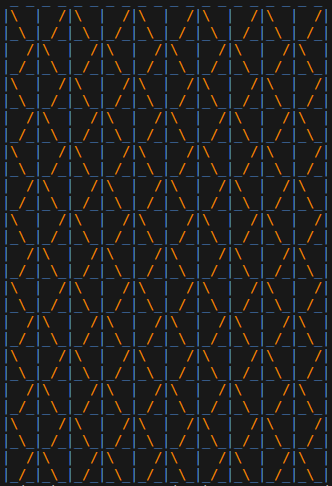
\includegraphics[width=0.4\linewidth]{maillage.png}
    \captionof{figure}{Affichage du maillage $N \times M = 10 \times 14$ dans le terminal}
\end{center}
\end{reponse}

%%%%%%%%%%%%%%%%%%%%%%%%%%%%%%%%%%%%%%%%%%%%%%%%%%%%%%%%%%%%%%%%%%%%%%%%%%%%%%%%

\begin{reponse}{31}

Soient $h_1 = \frac{2a}{N}, h_2 = \frac{2b}{M}$ et $h=\max(h_1,h_2)$. Soit $(x,y) \in \Omega$ quelconque. Alors en particulier, $x \in \, ]-a,a \,[$ et $y \in \, ]-b,b\,[$. Ainsi,

\begin{align*}
    x \in \, ]-a,a \,[ \quad & \Longleftrightarrow \quad -a<x<a \quad \Longleftrightarrow \quad 0<x+a<2a \\
    &\Longleftrightarrow \quad 0 < \frac{x+a}{h_1} < N \quad \Longleftrightarrow \quad 0<i<N.
\end{align*}

D'où $i \leq N-1$. De la même manière,

\begin{align*}
    y \in \, ]-b,b \,[ \quad & \Longleftrightarrow \quad -b<y<b \quad \Longleftrightarrow \quad 0<y+b<2b \\
    &\Longleftrightarrow \quad 0 < \frac{y+b}{h_2} < M \quad \Longleftrightarrow \quad 0<j<M.
\end{align*}

Ce qui donne $j \leq M-1$. \\ \\
Par définition de la partie entière,

\begin{align*}
    i = \operatorname{E}\left[\frac{x+a}{h_1}\right] & \Longrightarrow i \leq \frac{x+a}{h_1} < i+1 \\
    & \Longleftrightarrow \quad ih_1 \leq x+a \leq (i+1)h_1 \\ \\
    &\Longleftrightarrow \quad -a+ih_1 \leq x < -a+(i+1)h_1 \\ \\
    & \Longleftrightarrow \quad x_i \leq x < x_{i+1}.
\end{align*}

De manière analogue,

\begin{align*}
    j = \operatorname{E}\left[\frac{y+b}{h_2}\right] & \Longrightarrow j \leq \frac{y+b}{h_2} < j+1 \\
    & \Longleftrightarrow \quad jh_2 \leq y+b \leq (j+1)h_2 \\ \\
    & \Longleftrightarrow \quad -b+jh_2 \leq y < -b+(j+1)h_2 \\ \\
    & \Longleftrightarrow \quad y_j \leq y < y_{j+1}.
\end{align*}

On en déduit donc que $(x,y) \in [x_i,x_{i+1}[ \, \times \,  [y_j,y_{j+1}[$. Or $[x_i,x_{i+1}[ \, \times \,  [y_j,y_{j+1}[ \, \subset \,  T_l \cup T_{l+1}$. En effet, d'après la numérotation des noeuds que l'on a réalisé dans la partie 2, les sommets de $T_l$ et $T_{l+1}$ avec $l=(N+1)j+i$ sont respectivement $\{ \, (x_i,y_j), (x_i, y_{j+1}), (x_{i+1}, y_j) \, \}$ et $\{ \, (x_i,y_{j+1}), (x_{i+1}, y_{j+1}), (x_{i+1}, y_j) \, \}$ (ou bien $\{ \, (x_i,y_j), (x_i, y_{j+1}), (x_{i+1}, y_{j+1}) \, \}$ et $\{ \, (x_i,y_j), (x_{i+1}, y_{j+1}), (x_{i+1}, y_j) \, \}$ selon le sens de la partition du rectangle) :

\begin{center}
\begin{tikzpicture}[scale=2.5]
    \def\w{1.8}
    \def\h{0.9}
    \draw [thick] (0,0) rectangle (\w,\h);
    \draw [draw=purple!80!black, thick] (0,\h) -- (\w,0);
    \node [text=black, font=\large] at (\w*0.3, \h*0.3) {$\boldsymbol{T_{l}}$};
    \node [text=black, font=\large] at (\w*0.7, \h*0.7) {$\boldsymbol{T_{l+1}}$};
    \node [text=purple!60!black, font=\footnotesize, below left] at (0,0) {$(x_i,y_j)$};
    \node [text=purple!60!black, font=\footnotesize, below right] at (\w,0) {$(x_{i+1},y_j)$};
    \node [text=purple!60!black, font=\footnotesize, above left] at (0,\h) {$(x_i,y_{j+1})$};
    \node [text=purple!60!black, font=\footnotesize, above right] at (\w,\h) {$(x_{i+1},y_{j+1})$};
    \node [left=2pt] at (0, \h/2) {$j$};
    \node [below=2pt] at (\w/2, 0) {$i$};
\end{tikzpicture}
\end{center}

On a donc $(x,y) \in \, T_l \cup T_{l+1}$ et donc $(x,y) \in \, T_l$ ou $(x,y) \in \, T_{l+1}$.

\end{reponse}

%%%%%%%%%%%%%%%%%%%%%%%%%%%%%%%%%%%%%%%%%%%%%%%%%%%%%%%%%%%%%%%%%%%%%%%%%%%%%%%%

\begin{reponse}{32}

\textbf{(a)} D'après la question 3,

\[
    u^p(x,y) = \frac{\cos (m \pi x) \cos (m \pi y)}{2m^2\pi^2 +1}
\]

Pour simplifier l'écriture, on pose $C=\frac{1}{2m^2\pi^2 +1}$. On a d'une part

\[
    \frac{\partial u^p}{\partial x}(x,y) = -Cm\pi\sin(m \pi x)\cos(m\pi y),
\]

et d'autre part

\[
    \frac{\partial u^p}{\partial y}(x,y) = -Cm\pi\cos(m \pi x)\sin(m\pi y).
\]

On calcule ensuite les dérivées secondes :

\[
    \frac{\partial ^2u^p}{\partial x^2}(x,y) = -Cm^2\pi^2\cos (m\pi x)\cos(m\pi y) = -m^2\pi^2 u^p(x,y)
\]

et

\[
    \frac{\partial ^2u^p}{\partial y^2}(x,y) =-m^2\pi^2 u^p(x,y).
\]

On pose $\eta \, (x,y) = 1- \frac{\eta_0}{4}(x^2+y^2)$. Ainsi,

\[
    \frac{\partial}{\partial x}\left(\eta \frac{\partial u^p}{\partial x}\right)(x,y) = \frac{\eta_0x}{2}Cm\pi \sin(m \pi x) \cos(m \pi y) - m² \pi^2 u^p(x,y)\eta \, (x,y) := A(x,y)
\]

et

\[
        \frac{\partial}{\partial y}\left(\eta \frac{\partial u^p}{\partial y}\right)(x,y) = \frac{\eta_0x}{2}Cm\pi \cos(m \pi x) \sin(m \pi y) - m² \pi^2 u^p(x,y)\eta \, (x,y) := B(x,y).
\]

En reprenant l'équation (1) du sujet, avec $\lambda = 1$, on obtient alors

\begin{align*}
   & -\frac{\partial}{\partial x} \left( \eta \frac{\partial u^p}{\partial x}\right)(x,y) -\frac{\partial}{\partial y} \left( \eta \frac{\partial u^p}{\partial y}\right)(x,y) + \lambda u^p(x,y) = f(x,y) \\ \\
   \Longleftrightarrow \quad & f(x,y) = - A(x,y) - B(x,y) + u^p(x,y)
\end{align*}

En remplaçant $A(x,y)$ et $B(x,y)$ par leur expression donnée plus haut puis en factorisant, on obtient finalement :

\begin{align*}
    f(x,y) = -\frac{\eta_0 m \pi}{4m^2\pi^2 + 2}(x\sin(m\pi x)\cos(m\pi y)+ & y\cos(m\pi x)\sin(m\pi y)) \\
    & +(2m^2\pi^2\eta\,(x,y)+1)u^p(x,y).
\end{align*}

%%%%%%%%%%%%%%%%%%%%%%%%%%%%%%%%%%%%%%%%%%%%%%%%%%%%%%%%%%%%%%%%%%%%%%%%%%%%%%%%
\vspace{0.8em}
\textbf{(c)} En testant pour $m=1.$ et $N=M=2/h \in \{\,4,8,16,20,32,64,128 \,\}$, nous avons obtenu les erreurs relatives suivantes :

\begin{codeblock}
N e0 e1 e2
4 0.00137758 0.00137758 0.00137758
8 0.0425056 0.132984 0.0691583
16 0.00954852 0.0656942 0.022318
20 0.00602898 0.052484 0.0146806
32 0.00232045 0.032755 0.00590366
64 0.000575973 0.0163662 0.00149802
128 0.000143869 0.0081817 0.000378497
\end{codeblock}

\vspace{0.8em}

Avec le passage au log et un test sur un plus grand nombre de valeurs de $N$, cela nous a permis d'obtenir le graphe suivant :

\begin{center}
    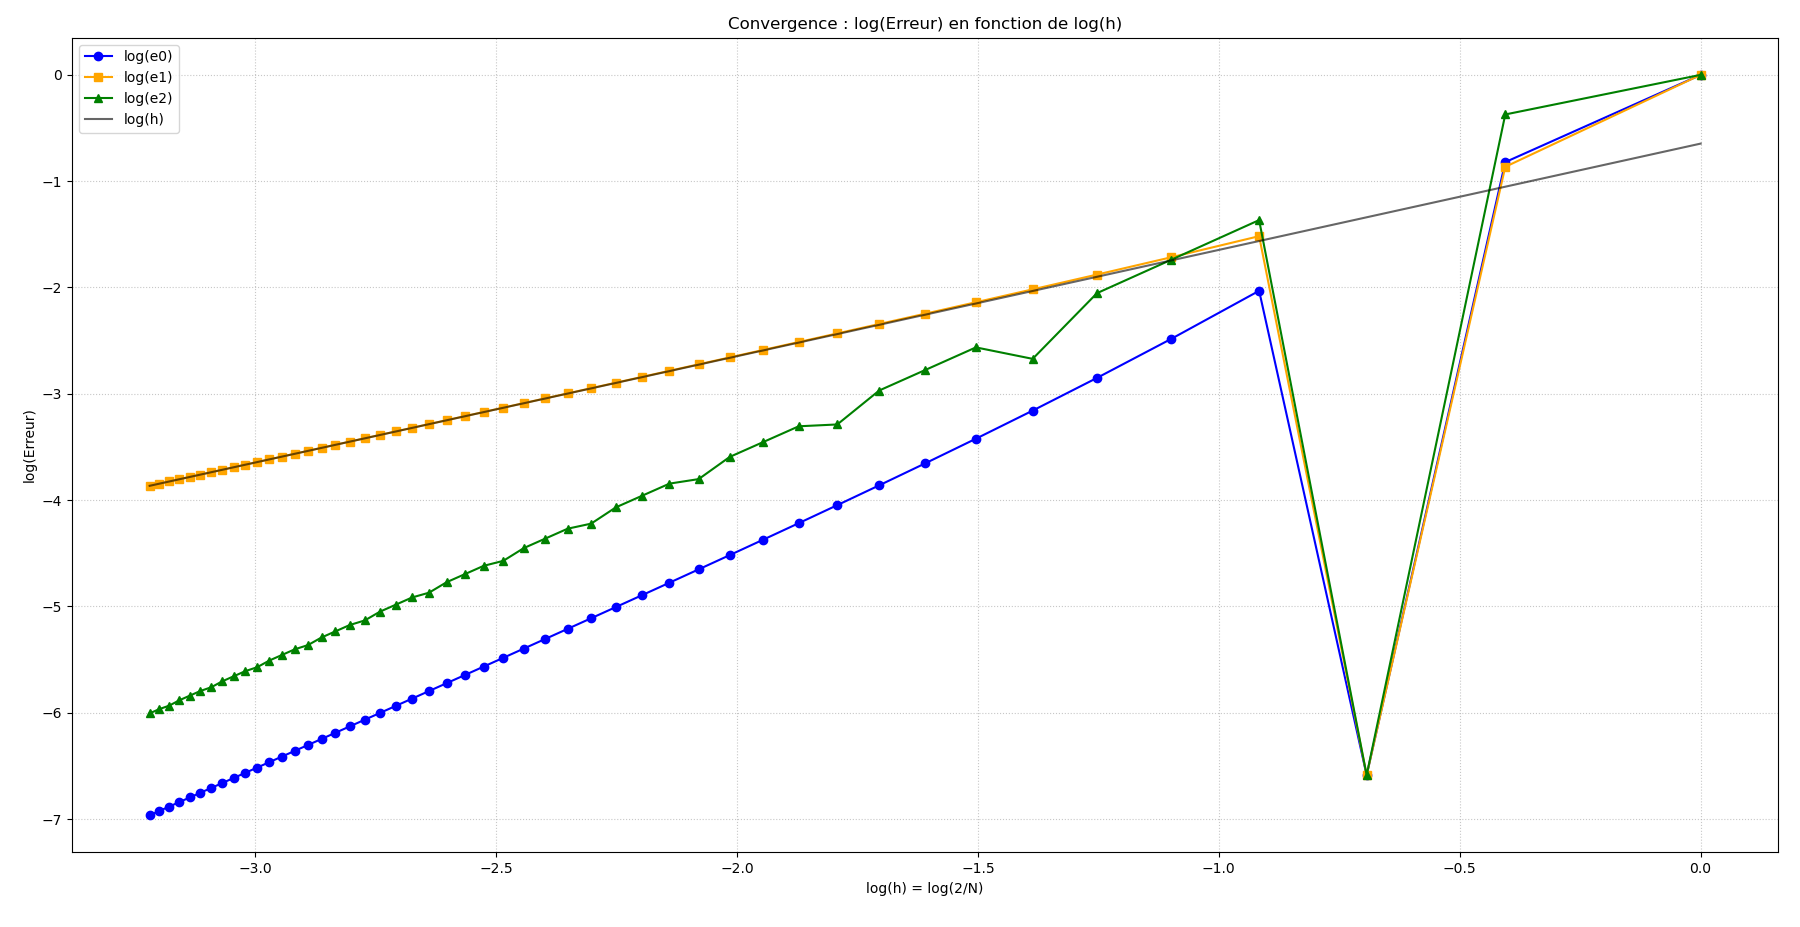
\includegraphics[width=1\linewidth]{erreurs.png}
    \captionof{figure}{Tracé des courbes d'erreurs}
\end{center}

\vspace{0.8em}

On remarque que pour $N=4$, l'erreur plonge, ce qui indique que la solution approchée correspond presque exactement à la solution réelle : les noeuds du maillage semblent donc coïncider avec les points de la solution exacte.

%%%%%%%%%%%%%%%%%%%%%%%%%%%%%%%%%%%%%%%%%%%%%%%%%%%%%%%%%%%%%%%%%%%%%%%%%%%%%%%%
\vspace{1.6em}
\textbf{(d)} A partir de la question 31, nous avons pu créer une fonction eval\_uh que nous avons évalué en 50 points pour différentes valeurs de $m$. En comparant avec la fonction log(h), nous avons obtenu les graphes suivants :

\begin{center}
    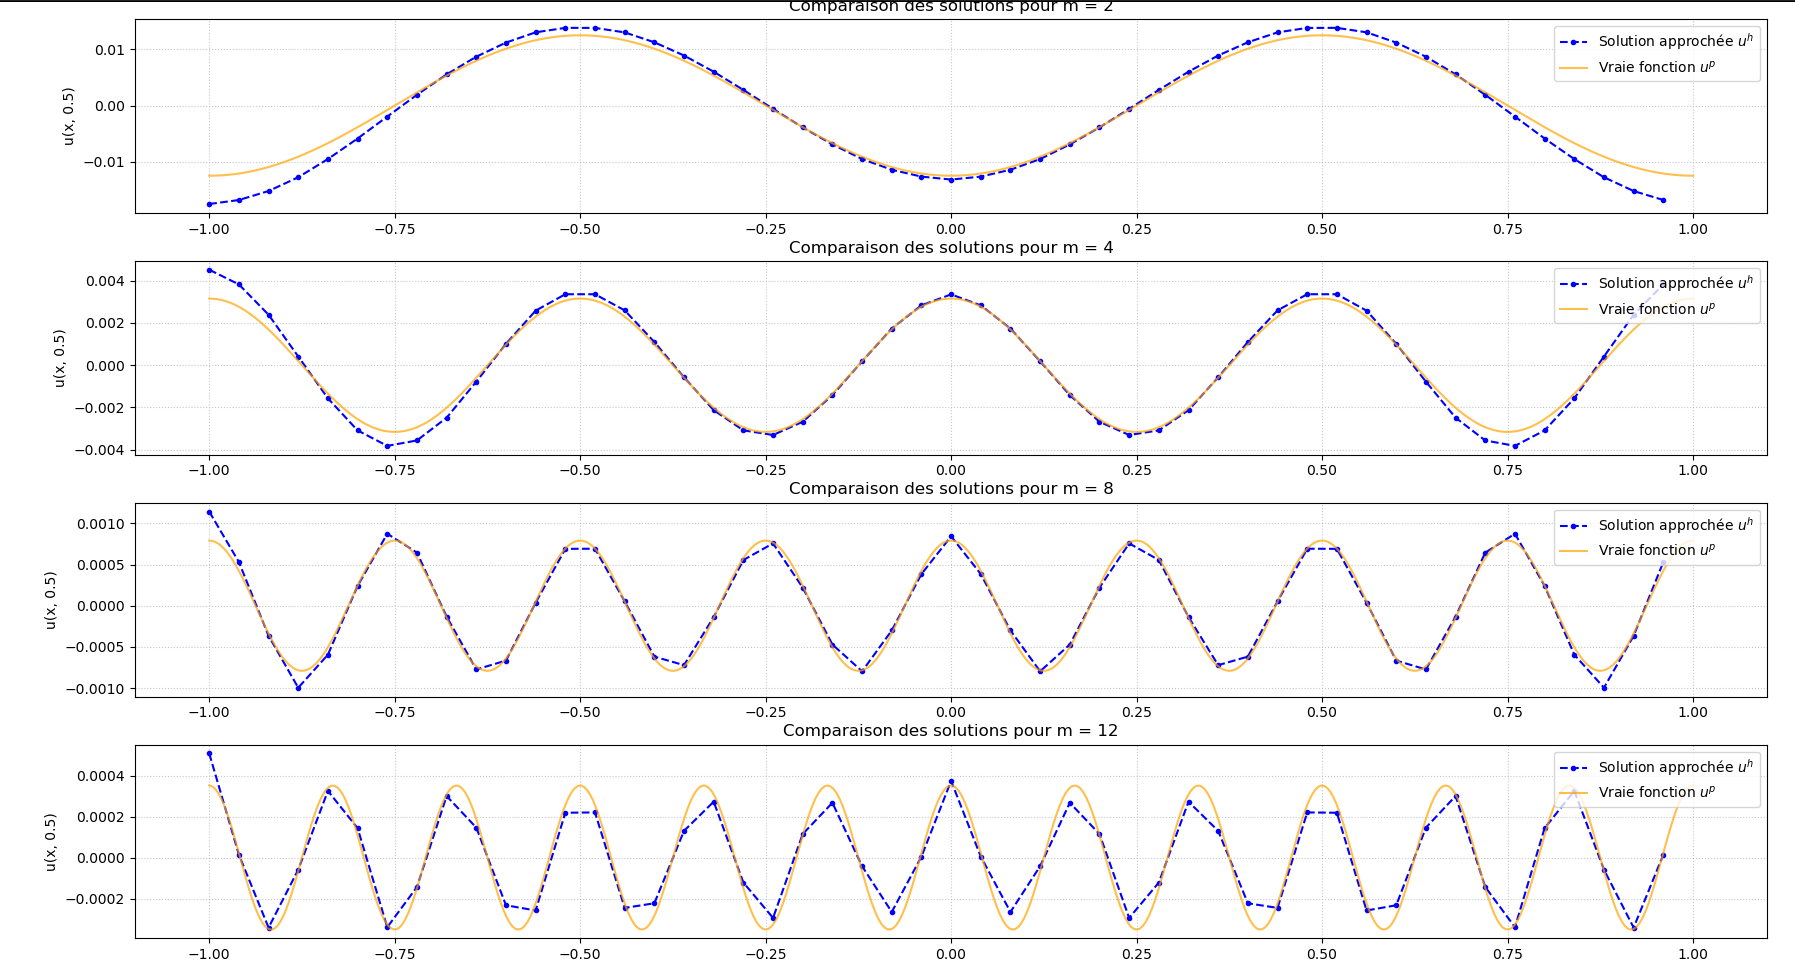
\includegraphics[width=1\linewidth]{graphes.png}
    \captionof{figure}{Tracé des courbes pour $x \in [-1,1]$}
\end{center}

\vspace{0.8em}

On observe que pour des petites valeurs de m ($2,4$) le maillage $N=32$ est suffisant, mais lorsque $m$ grandit, le maillage n'est plus assez fin pour capter les variations de la fonction, et donc l'erreur est bien plus grande.

\end{reponse}

\newpage

\chapter{Structure du programme}

La structure du code étant un élément essentiel dans un projet, nous y avons porté un soin tout particulier. Il est structuré en trois fichiers principaux : \hyperref[sec:fonctions]{fonctions.cpp}, \hyperref[sec:main]{main.cpp} et \hyperref[sec:tests]{tests.cpp}; contenant respectivement les fonctions relatives au projet, les tests numériques et des tests pour la plupart des fonctions codées. \\

Afin de structurer davantage notre code, nous avons opté pour l'utilisation de classes. Ce choix à engendré bien des questionnements notamment sur la manière de définir nos classes et la pertinence réelle de leur utilisation dans ce projet. Nous n'avons au final, eu l'utilité que d'une seule, la classe \hyperref[sec:triangle]{triangle.cpp}. Elle nous a permis, entre autres, de plus agréablement manipuler les maillages, qui n'est représenté maintenant que par un tableau de Triangle au lieu d'une matrice. Cette classe est défini par ses 3 attributs : $n1, n2, n3$ qui correspondent au trois sommets, avec la numérotation des noeuds dans le maillage. La surcharge de l'opérateur == permet une comparaison plus pratique des triangles (cette surcharge est presque obligatoire pour faire les tests dans de bonnes conditions). \\ 

Nous avons également fourni un fichier \hyperref[secsec:tests]{tests.cpp}, comme annoncé au début du paragraphe, pour s'assurer que les fonctions codées tout au long du projet, soient correctes et donc que nous travaillons sur de bonnes bases. \\

Toutes nos tentatives ne sont pas utilisées dans la version finale. La première aura été de créer une classe noeud.cpp, que nous avons enlevé faute d'utilité et cela s'explique par la très bonne numérotation des sommets dans le maillage qui est autosuffisante. La deuxième est la classe \hyperref[sec:vh]{elementvh.cpp} qui est visible dans le code en annexe. Encore une fois, la manière proposée d'aborder le problème nous a paru plus appropriée et moins lourde que l'utilisation d'une classe. Dans ce que nous visualisions, nous l'utilisions que dans une seule fonction (cf. \ref{sec:vh}), ce qui justifie son retrait.

\newpage

\chapter{Annexe A : main}

L'annexe ci-dessous contient la fichier principal du programme. En particulier, nous y avons inclut les fonctions spécifiques aux tests numériques (affichage du maillage, évaluation de $u^h$ en un point de $\Omega$, $\dots$) et à la génération des .txt à partir desquels nous avons pu visualiser nos résultats (questions 30, 32(c) et 32(d)).

\begin{codeblock}[main.cpp]
#include <iostream>
#include <cmath>
#include <fstream>

#include <functional>

#include "fonctions.hpp"

using namespace std;

const string BLEU  = "\033[34m";
const string ORANGE = "\033[38;5;208m";
const string BLANC = "\033[0m";

void affiche_maillage(int N, int M){

    cout << "Affichage du maillage pour N = "<< N << ", M = "<<M<<".\n";

    // Affichage de la première ligne
    string buffer_haut ="" + BLEU;
    for (int c = 0; c < N; c++) buffer_haut += " _ _";

    buffer_haut += BLANC + "\n";
    cout << buffer_haut ;

    for (int l = M-1; l >= 0; l--){

        string buffer_mil = "";
        string buffer_bas = "";

        for (int c = 0; c < N; c++){

            bool direction = ((l + c) % 2 == 0);

            if (c == 0){
                buffer_mil += BLEU + "|" + BLANC;
                buffer_bas += BLEU + "|" + BLANC;
            }

            if (direction){ // CAS 1 : direction "croissante"
                buffer_mil += ORANGE + "  /" + BLEU + "|" + BLANC;
                buffer_bas += BLEU + "_"+ ORANGE +"/" + BLEU + "_|" + BLANC;
            } else {  // CAS 2 : direction "décroissante"
                buffer_mil += ORANGE + "\\  "+ BLEU + "|"+ BLANC ;
                buffer_bas += BLEU + "_"+ ORANGE +"\\"+BLEU + "_|" + BLANC;
            }
       }

        cout << buffer_mil << endl << buffer_bas << endl;
    }

}


double up(double x, double y, int m){
    double c = (2.*m*m*M_PI*M_PI + 1);
    return (cos(m*M_PI*x)*cos(m*M_PI*y)) /c ;
}

// Se référer à la question 32)a. Pour la formule
double f(double x, double y, int m, double eta0, double (* eta) (double,double)){
    double k = -(eta0*m*M_PI)/(4.*m*m*M_PI*M_PI +2);
    double t = x*sin(m*M_PI*x)*cos(m*M_PI*y) + y*cos(m*M_PI*x)*sin(m*M_PI*y);
    double o = 2*m*m*M_PI*M_PI*eta(x,y) +1;
    return k*t + o*up(x,y,m);
}

// Cas eta0=0
double f0(double x, double y, int m){
    return f(x,y,m,0,[](double,double){return 1.;});
}

// Cas eta0=1
double f1(double x, double y, int m){
    return f(x,y,m,1.,[](double,double){return 1.;});
}

double eta(double eta0, double x, double y){
    return 1. - eta0/4 * (x*x+y*y);
}

double eval_uh(double x, double y, vector<double> uh, maillage TRG, int N, int M, double a, double b){
    // On cherche à identifier dans quel triangle se trouve (x,y)
    double h1 = (2*a)/N;
    double h2 = (2*b)/M;
    int i = (int) ((x+a)/h1);
    int j = (int) ((y+b)/h2);

    int l = 2*j*N+2*i;

    // (x,y) est dans T_l ou T_{l+1} (q31)
    // On a besoin du signe des lambdas

    for (int t = l; t < l + 2; t++){
        Triangle T = TRG[t];

        duplix xs_ys = CoordsTrig(a, b, N, M, T);
        vector<double> xs = get<0>(xs_ys);
        vector<double> ys = get<1>(xs_ys);

        matrix BT = CalcMatBT(xs, ys);

        double detBT = BT[0][0]*BT[1][1] - BT[0][1]*BT[1][0];

        // Inversion BT
        matrix inv_BT = {{BT[1][1]/detBT, -BT[0][1]/detBT},
                        {-BT[1][0]/detBT, BT[0][0]/detBT}};

        // Calcul des lambdas
        double lambda_1 = inv_BT[0][0]*(x - xs[0]) + inv_BT[0][1]*(y - ys[0]);
        double lambda_2 = inv_BT[1][0]*(x - xs[0]) + inv_BT[1][1]*(y - ys[0]);
        double lambda_0 = 1. - lambda_1 - lambda_2;

        // Test signe
        if (lambda_0 >= 0 && lambda_1 >= 0 && lambda_2 >= 0){

            // Alors (x,y) est dans ce triangle
            double eval = lambda_0*uh[T.get(0)] + lambda_1*uh[T.get(1)] + lambda_2*uh[T.get(2)];

            return eval;
        }
    }

    return 0.;
}

int main(){
    cout << "Début des tests numériques\n";

    // Déclaration des paramètres
    const double a = 1.;
    const double b = 1.;
    int m = 1;

    auto lambda = [](double,double){ return 1.;};

    auto eta1 = lambda;

    // Tests numériques

    affiche_maillage(10,14);

    vector<int> valeurs_tests = {4,8,16,20,32,64};
    vector<int> valeurs_tests1(49);
    for (int k = 0; k < 49;k++) valeurs_tests1[k] = k+2;

    // Création d'un fichier, pour stocker les erreurs pour l'affichage

    ofstream fichier("erreurs.txt");
    ofstream fichier2("log_erreurs.txt");
    if (!fichier.is_open() || !fichier2.is_open()) {
        cout << "Erreur lors de l'ouverture d'un fichier.\n";
        return 1;
    }

    fichier << "N e0 e1 e_2\n";
    fichier2 << "N log(e0) log(e1) log(e_2)\n";

    // Calculs pour la question 32(c)
    cout << "Calcul des erreurs en cours...\n";

    for (int N : valeurs_tests1){
        maillage maillageNxN = maillageTR(N,N);

        vector<double> B = scdmembre(f0,N,N,maillageNxN,a,b,m);

        vector<double> uh = bicg_stab(B,maillageNxN,N,N,a,b,1e-10,100000,eta1);

        auto up0 = [](double x, double y, int m){ return up(x,y,m);};
        vector<double> tab_err = erreurs(up0,uh,maillageNxN,N,N,a,b,m);
        vector<double> tab_log_err(tab_err.size());

        for (int i = 0; i < tab_log_err.size(); i++){
            tab_log_err[i] = log(tab_err[i]);
        }

        cout << "log(e0(2/" << N << ")) = " << tab_log_err[0] << ", ";
        cout << "log(e1(2/" << N << ")) = " << tab_log_err[1] << ", ";
        cout << "log(e2(2/" << N << ")) = " << tab_log_err[2] << ", ";
        cout << "log(2/" << N << ") = " << log(2./N) << endl;

        cout << "e0(2/" << N << ") = " << tab_err[0] << ", ";
        cout << "e1(2/" << N << ") = " << tab_err[1] << ", ";
        cout << "e2(2/" << N << ") = " << tab_err[2] << " \n";

        fichier << N << " " << tab_err[0] << " " << tab_err[1] << " " << tab_err[2] << "\n";
        fichier2 << N << " " << tab_log_err[0] << " " << tab_log_err[1] << " " << tab_log_err[2] << "\n";
    }

    // Début de tests question 32(d), maillage 32x32, 50 points par courbe

    cout << "Génération des courbes en cours...\n";

    ofstream fichier1("courbes.txt");
    if (!fichier1.is_open()) {
        cout << "Erreur lors de l'ouverture du fichier.\n";
        return 1;
    }

    fichier1 << "m x u^h u^p\n";
    double pas = 2./50;
    int N_courbes = 32;

    maillage maillage_courbes = maillageTR(N_courbes, N_courbes);

    // Tests sur differentes valeurs de m
    vector<int> valeurs_m = {2, 4, 8, 12};

    for (int m_courbe : valeurs_m){
        auto f1_courbe = [](double x, double y, int m_courbe){ return f1(x, y, m_courbe);};
        vector<double> B_courbe = scdmembre(f1_courbe, N_courbes, N_courbes, maillage_courbes, a, b, m_courbe);

        auto eta1_courbe = [](double x, double y){return eta(1.,x,y);};
        vector<double> uh_courbe = bicg_stab(B_courbe, maillage_courbes, N_courbes, N_courbes, a, b, 1e-10, 100000, eta1_courbe);

        double ctr = -1.;

        while (ctr <= 1.){
            double u_app = eval_uh(ctr, 0.5, uh_courbe, maillage_courbes, N_courbes, N_courbes, a, b);
            double u_exa = up(ctr, 0.5, m_courbe);

            fichier1 << m_courbe << " " << ctr << " " << u_app << " " << u_exa << "\n";
            ctr += pas;
        }

    }

    cout << "Tests terminés, les fichiers .txt sont prêts !\n";

}
\end{codeblock}

\newpage

\chapter{Annexe B : fonctions}

L'annexe ci-dessous contient toutes les fonctions demandées dans les questions qui n'apparaissent pas explicitement dans le chapitre "Réponses aux questions théoriques" (cf. remarques en début de chaque partie du chapitre sus-mentionné). Nous avons pris la liberté d'ajouter quelques fonctions supplémentaires pour en alléger d'autres.

\begin{codeblock}[fonctions.hpp]
#ifndef FONCTIONS_H
#define FONCTIONS_H

#include <tuple>
#include <vector>


#include "triangle.hpp"

using namespace std;

typedef vector<vector<double>> matrix;
typedef tuple<vector<double>,vector<double>> duplix;
typedef vector<Triangle> maillage;

vector<double> Subdiv(double a, int N);

int numgb(int N, int M, int i, int j);

tuple<int,int> invnumgb(int N, int M,int s);

maillage maillageTR(int N, int M);

duplix CoordsTrig(double a, double b, int N,int M, Triangle T);

matrix CalcMatBT(vector<double> xs, vector<double> ys);

vector<double> integ_eta_triang(double (* eta)(double,double),
    maillage TRG,int N, int M,double a,double b);

matrix DiffTerm(duplix xs_ys, double val);

matrix ReacTerm(duplix xs_ys);

vector<double> matvec(vector<double> V, maillage TRG, int N, int M,
    double a, double b, double (* eta)(double,double));

#endif

vector<double> scdmembre(double rhsf(double,double, int), int N, int M, maillage TRG, double a, double b, int m);

double normL2(vector<double> V,maillage TRG, int N, int M, double a, double b);

double normL2Grad(vector<double> V, maillage TRG, int N, int M, double a, double b);

double pdt_sc(vector<double> u, vector<double> v);

vector<double> cl_vec(double lbd, vector<double> u, double mu, vector<double> v);

double max_abs(vector<double> V);

vector<double> bicg_stab(vector<double> B,maillage TRG, int N, int M, double a,
    double b, double tol,int max_it, double (* eta) (double,double));

vector<double> erreurs(double (* solExa) (double,double, int),vector<double> uh,maillage TRG, int N, int M, double a, double b, int m);
\end{codeblock}

\begin{codeblock}[fonctions.cpp]
#include <stdlib.h>
#include <cmath>

#include "fonctions.hpp"



// Fonction qui renvoie une subdivision uniforme de [-a,a]
vector<double> Subdiv(double a, int N){
    vector<double> subdiv = vector<double>(N+1);
    double pas = 2*a / N;

    for (int k = 0; k <= N; k++) subdiv[k] = -a + k*pas;

    return subdiv;
}

// Fonction qui renvoie le numéro associé à des coordonnées
int numgb(int N, int M, int i, int j){ return (N+1)*j + i; }

//Fonction qui étant donné entier s valide, donne les coordonnées du noeud
tuple<int,int> invnumgb(int N, int M,int s){
    return {s % (N+1),s / (N+1)};
}

//Fonction qui étant donné un pavé de NM rectangles renvoie un TRG
//triangulaire sous forme d'une liste qui contient les triangles
maillage maillageTR(int N, int M){
    maillage TRG(2*N*M);
    int k = 0;
    bool direction = true; // true pour "/" et false pour "\"

    for (int l = 0; l < M; l++){
        for (int c = 0; c < N ; c++){

            //Pour alterner le sens des triangles à chaque petit rectangle
            direction = (l+c)%2 == 0;

            // Calcul des coordonnées des quatres sommets du rectangle
            int bas_g = numgb(N,M,c,l);
            int bas_d = numgb(N,M,c+1,l);
            int haut_g = numgb(N,M,c,l+1);
            int haut_d = numgb(N,M,c+1,l+1);

            // Création des triangles
            if (direction){
                TRG[k] = Triangle(bas_g,haut_g,haut_d);
                TRG[k+1] = Triangle(bas_g,bas_d,haut_d);
            } else {
                TRG[k] = Triangle(bas_g,haut_g,bas_d);
                TRG[k+1] = Triangle(haut_g,haut_d,bas_d);
            }

            k += 2;
        }
    }

    return TRG;
}


// Fonction qui renvoie les coordonnées des points du triangle
duplix CoordsTrig(double a, double b, int N,
    int M, Triangle T){
    vector<double> xs = vector<double>(3);
    vector<double> ys = vector<double>(3);

    for (int k = 0; k < 3; k++){
        tuple<int,int> tup = invnumgb(N,M,T.get(k));
        xs[k] = -a + (2*a)/N * get<0>(tup);
        ys[k] = -b + (2*b)/M * get<1>(tup);

    }

    return {xs,ys};
}


// Fonction qui renvoie la jacobienne de F_T
// Voir question 20, elle justifie ce calcul
matrix CalcMatBT(vector<double> xs, vector<double> ys){
    double bt_00 = xs[1] - xs[0];
    double bt_10 = ys[1] - ys[0];
    double bt_01 = xs[2] - xs[0];
    double bt_11 = ys[2] - ys[0];

    return {{bt_00,bt_01},{bt_10,bt_11}};
}




double integ_triangle(double (* f)(double,double), Triangle T,int N, int M,double a,double b){

    // Calcul du determinant de B_T
    duplix xs_ys = CoordsTrig(a,b,N,M,T);
    vector<double> xs = get<0>(xs_ys);
    vector<double> ys = get<1>(xs_ys);

    double det = abs((xs[1]-xs[0])*(ys[2]-ys[0]) - (ys[1]-ys[0])*(xs[2]-xs[0]));

    // On determine les milieux des côtes de T
    double m0x = (xs[0] + xs[1])/2.;
    double m0y = (ys[0] + ys[1])/2.;
    double m1x = (xs[1] + xs[2])/2.;
    double m1y = (ys[1] + ys[2])/2.;
    double m2x = (xs[0] + xs[2])/2.;
    double m2y = (ys[0] + ys[2])/2.;

    // Calculs de f \circ F_T en les milieux des côtés du triangles T^
    double f0 = f(m0x,m0y);
    double f1 = f(m1x,m1y);
    double f2 = f(m2x,m2y);

    return 1./6. * det * (f0 + f1 + f2);
}


vector<double> integ_eta_triang(double (* eta)(double,double),
    maillage TRG,int N, int M,double a,double b){

    vector<double> ET = vector<double>(TRG.size());
    int k =0;

    // Parcours du maillage
    for (Triangle T : TRG){


        ET[k] = integ_triangle(eta,T,N,M,a,b);
        k++;
    }

    return ET;
}


matrix DiffTerm(duplix xs_ys, double val){
    vector<double> xs = get<0>(xs_ys);
    vector<double> ys = get<1>(xs_ys);

    matrix BT = CalcMatBT(xs,ys);
    double det = (xs[1]-xs[0])*(ys[2]-ys[0]) - (ys[1]-ys[0])*(xs[2]-xs[0]);

    //Construction de la transposée de l'inverse de BT
    matrix trsp_inv_BT = {{0,0},{0,0}};
    trsp_inv_BT[0][0] = 1/det * BT[1][1];
    trsp_inv_BT[0][1] = -1/det * BT[1][0];
    trsp_inv_BT[1][0] = -1/det * BT[0][1];
    trsp_inv_BT[1][1] = 1/det * BT[0][0];


    //Calcul des Nabla_lambda^
    vector<double> NLcha0 = {{-1,-1}}; //lambdacha0 = (1-x^-y^)
    vector<double> NLcha1 = {{1,0}}; //lambdacha1 = x^
    vector<double> NLcha2 = {{0,1}}; //lambdacha2 = y^
    //Calcul des Nabla_lambda = BT*Nabla_lambdacha
    double nl00 = trsp_inv_BT[0][0] * NLcha0[0] + trsp_inv_BT[0][1] * NLcha0[1];
    double nl01 = trsp_inv_BT[1][0] * NLcha0[0] + trsp_inv_BT[1][1] * NLcha0[1];

    double nl10 = trsp_inv_BT[0][0] * NLcha1[0] + trsp_inv_BT[0][1] * NLcha1[1];
    double nl11 = trsp_inv_BT[1][0] * NLcha1[0] + trsp_inv_BT[1][1] * NLcha1[1];

    double nl20 = trsp_inv_BT[0][0] * NLcha2[0] + trsp_inv_BT[0][1] * NLcha2[1];
    double nl21 = trsp_inv_BT[1][0] * NLcha2[0] + trsp_inv_BT[1][1] * NLcha2[1];

    //Calcul des produits scalaires * ET
    double val00 = val * (nl00 * nl00 + nl01 * nl01);
    double val01 = val * (nl00 * nl10 + nl01 * nl11);
    double val02 = val * (nl00 * nl20 + nl01 * nl21);
    double val11 = val * (nl10 * nl10 + nl11 * nl11);
    double val12 = val * (nl10 * nl20 + nl11 * nl21);
    double val22 = val * (nl20 * nl20 + nl21 * nl21);

    return {{val00, val01, val02},
        {val01, val11, val12},
        {val02, val12, val22}
    };
}


matrix ReacTerm(duplix xs_ys){
    vector<double> xs = get<0>(xs_ys);
    vector<double> ys = get<1>(xs_ys);

    double det = (xs[1]-xs[0])*(ys[2]-ys[0]) - (ys[1]-ys[0])*(xs[2]-xs[0]);

    //Calcul des integrales des lambda_i * lambda_j
    double int_lambda_ii = abs(det) * 1.0/12.0;
    double int_lambda_ij = abs(det) * 1.0/24.0;

    return {{int_lambda_ii, int_lambda_ij, int_lambda_ij},
        {int_lambda_ij, int_lambda_ii, int_lambda_ij},
        {int_lambda_ij, int_lambda_ij,int_lambda_ii}};
}




vector<double> matvec(vector<double> V, maillage TRG, int N, int M,
    double a, double b, double (* eta)(double,double)){

    int K = 2*N*M;
    vector<double> W((N+1)*(M+1));

    // Contient les valeurs de l'integrales de eta sur chaque T
    vector<double> VALS = integ_eta_triang(eta,TRG, N,M,a,b);

    for (int t = 0; t < K; t++){
        Triangle T = TRG[t];

        // Calcul de B_T
        duplix xs_ys = CoordsTrig(a,b,N,M,T);
        matrix D = DiffTerm(xs_ys,VALS[t]);
        matrix R = ReacTerm(xs_ys);

        for (int i = 0; i < 3; i++){
            int k = T.get(i);

            // Calcul de la contribution
            double res = 0;

            for (int r = 0; r < 3; r++){
                int j = T.get(r);

                // aT = Diff + Reac
                double PROD2 = D[r][i]+R[r][i];
                res += V[j] * PROD2;
            }

            W[k] += res;
        }
    }

    return W;
}



vector<double> scdmembre(double rhsf(double,double,int), int N, int M, maillage TRG,
    double a, double b, int m){

    vector<double> B((N+1)*(M+1));
    int K = 2*N*M;

    for (int t = 0; t < K; t++){

        duplix xs_ys = CoordsTrig(a,b,N,M,TRG[t]);
        vector<double> xs = get<0>(xs_ys);
        vector<double> ys = get<1>(xs_ys);

        double det = abs((xs[1]-xs[0])*(ys[2]-ys[0]) - (ys[1]-ys[0])*(xs[2]-xs[0]));

        // calcul des milieux
        double m0x = (xs[0] + xs[1])/2.;
        double m0y = (ys[0] + ys[1])/2.;
        double m1x = (xs[1] + xs[2])/2.;
        double m1y = (ys[1] + ys[2])/2.;
        double m2x = (xs[0] + xs[2])/2.;
        double m2y = (ys[0] + ys[2])/2.;

        // Calculs de (f \circ F_T)*(w \circ F_T) en les milieux des côtés du triangles T^
        double f0 = rhsf(m0x,m0y,m);
        double f1 = rhsf(m1x,m1y,m);
        double f2 = rhsf(m2x,m2y,m);

        // Calcul des contributions des sommets de T aux noeuds
        B[TRG[t].get(0)] += (det * (f0*0.5 + f2*0.5))/6;
        B[TRG[t].get(1)] += (det * (f0*0.5 + f1*0.5))/6;
        B[TRG[t].get(2)] += (det * (f1*0.5 + f2*0.5))/6;
    }

    return B;
}


double normL2(vector<double> V,maillage TRG, int N, int M, double a, double b){

    int K = 2*N*M;
    int G = (N+1)*(M+1);
    vector<double> W(G);

    // Calcul de AV
    for (int t = 0; t < K; t++){
        Triangle T = TRG[t];

        duplix xs_ys = CoordsTrig(a,b,N,M,T);
        matrix R = ReacTerm(xs_ys);

        for (int i = 0; i < 3; i++){
            int k = T.get(i);

            // Calcul de la contribution
            double res = 0;

            for (int r = 0; r < 3; r++){
                int j = T.get(r);

                // aT = Diff + Reac (mais Diff = 0 car eta = 0)
                res += V[j] * R[r][i];
            }

            W[k] += res;
        }
    }

    // Calcul de V^T * (AV)
    double norme_carre = 0;
    for (int k = 0; k < G; k++)
        norme_carre += V[k]*W[k];

    return sqrt(norme_carre);
}


double normL2Grad(vector<double> V, maillage TRG, int N, int M, double a,
    double b){

    int K = 2*N*M;
    int G = (N+1)*(M+1);
    vector<double> W(G);

    // Contient les valeurs de l'integrales de eta sur chaque T
    vector<double> VALS = integ_eta_triang([](double,double){return 1.;},TRG, N,M,a,b);

    // Calcul de AV
    for (int t = 0; t < K; t++){
        Triangle T = TRG[t];

        duplix xs_ys = CoordsTrig(a,b,N,M,T);
        matrix D = DiffTerm(xs_ys,VALS[t]);

        for (int i = 0; i < 3; i++){
            int k = T.get(i);

            // Calcul de la contribution
            double res = 0;

            for (int r = 0; r < 3; r++){
                int j = T.get(r);

                // aT = Diff + Reac (mais reac = 0 car lambda = 0)
                res += V[j] * D[r][i];
            }

            W[k] += res;
        }
    }

    // Calcul de V^T * (AV)
    double norme_carre = 0;
    for (int k = 0; k < G; k++)
        norme_carre += V[k]*W[k];

    return sqrt(norme_carre);
}

// Fonction qui calcule le produit scalaire de deux vecteurs
double pdt_sc(vector<double> u, vector<double> v){
    double prod = 0;
    int N = u.size();

    for (int k = 0; k < N; k++){
        prod += u[k]*v[k];
    }

    return prod;
}

// Fonction qui renvoie la combinaison linéaire de deux vecteurs
vector<double> cl_vec(double lbd, vector<double> u, double mu, vector<double> v){
    int L = u.size();
    vector<double> cl(L);

    for (int k = 0; k < L; k++){
        cl[k] = lbd*u[k] + mu*v[k];
    }

    return cl;
}


// Fonction qui renvoie la composante max en valeur absolue d'un vecteur
double max_abs(vector<double> V){
    double max = V[0];

    for (double x : V)
        if (abs(x) > max) max = abs(x);

    return max;
}

vector<double> bicg_stab(vector<double> B,maillage TRG, int N, int M, double a,
    double b, double tol,int max_it, double (* eta) (double,double)){

    vector<double> AW,AS,S,R_tmp;
    vector<double> X((N+1)*(M+1),0);

    // on choisit X0=0 (ca nous évite un prod mat vec)
    vector<double> R = B;
    vector<double> R_etoile = R;


    vector<double> W = R;
    int it = 0;

    // Itérations, bicg_stab selon l'algorithme donné
    while (max_abs(R) > tol && it < max_it){
        AW = matvec(W,TRG,N,M,a,b,eta);
        double alpha = pdt_sc(R,R_etoile) / pdt_sc(AW,R_etoile);

        S = cl_vec(1.,R,-alpha,AW);

        AS = matvec(S,TRG,N,M,a,b,eta);
        double omega = pdt_sc(AS,S)/pdt_sc(AS,AS);

        // Actualisation des variables pour le prochain tour de boucle
        X = cl_vec(1.,X,1.,cl_vec(alpha,W,omega,S));
        R_tmp = R;
        R = cl_vec(1.,S,-omega,AS);

        double beta = (pdt_sc(R,R_etoile) * alpha) / (pdt_sc(R_tmp,R_etoile) * omega);
        W = cl_vec(1.,R,beta,cl_vec(1.,W,-omega,AW));
        it++;
    }

    return X;
}


vector<double> erreurs(double (* solExa) (double,double, int),vector<double> uh,
    maillage TRG, int N, int M, double a, double b, int m){

    vector<double> tab_err(3);
    int G = (N+1)*(M+1);

    vector<double> uchap(G);

    for (int s = 0; s < G; s++){
        tuple<int,int> coord_noeud = invnumgb(N,M,s);
        double x = -a + (2*a)/N * get<0>(coord_noeud);
        double y = -b + (2*b)/M * get<1>(coord_noeud);

        uchap[s] = solExa(x,y,m);
    }


    vector<double> diff = cl_vec(1.,uchap,-1.,uh);

    tab_err[0] = normL2(diff,TRG,N,M,a,b) / normL2(uchap,TRG,N,M,a,b);
    tab_err[1] = normL2Grad(diff,TRG,N,M,a,b) / normL2Grad(uchap,TRG,N,M,a,b);
    tab_err[2] = max_abs(diff) / max_abs(uchap);

    return tab_err;
}
\end{codeblock}

\newpage

\chapter{Annexe C : classe Triangle}

Le code ci-dessous permet de créer la classe Triangle, entièrement définie par le numéro de ses sommets dans le maillage. Elle comprend également un getter qui renvoie le numéro du sommet demandé. Nous avons également surchargé l'opérateur == afin de facilité les tests.

\begin{codeblock}[triangle.hpp]
#ifndef TRIANGLE_H
#define TRIANGLE_H

class Triangle {

private:
    int n1, n2, n3;

public:
    Triangle(int n1, int n2, int n3);
    Triangle();
    int get(int k);

    // Surcharge de ==
    bool operator==(const Triangle &autre) const;
};


#endif
\end{codeblock}

\begin{codeblock}[triangle.cpp]
#include "triangle.hpp"


Triangle::Triangle(int n1, int n2, int n3){
    this->n1 = n1;
    this->n2 = n2;
    this->n3 = n3;
}


Triangle::Triangle(){
    this->n1 = 0;
    this->n2 = 0;
    this->n3 = 0;
}


int Triangle::get(int k){
    switch (k){
        case 0 : return this->n1;
        case 1 : return this->n2;
        case 2 : return this-> n3;
        default : return -1;
    }
}

// Fonction qui renvoie le min de 3 entiers
int min3(int a, int b, int c) {
    int m = (a < b) ? a : b;
    return (m < c) ? m : c;
}


// Fonction qui renvoie le max de 3 entiers
int max3(int a, int b, int c) {
    int m = (a > b) ? a : b;
    return (m > c) ? m : c;
}


// Surcharge de l'opérateur == pour définir l'égalité de triangles
bool Triangle::operator==(const Triangle &t) const {
    int min1 = min3(n1,n2,n3);
    int max1 = max3(n1,n2,n3);
    int mid1 = n1 + n2 + n3 - min1 - max1;

    int min2 = min3(t.n1,t.n2,t.n3);
    int max2 = max3(t.n1,t.n2,t.n3);
    int mid2 = t.n1 + t.n2 + t.n3 - min2 - max2;

    return min1==min2 && mid1==mid2 && max1==max2;
}
\end{codeblock}

\newpage

\chapter{\, Annexe D : classe ElementVh}

\label{sec:vh}
Le code ci-dessous permet de créer la classe ElementVh, comme suggéré en remarque en début de partie 3. Elle comprend des fonctions get, permettant de récupérer ses différentes propriétés. Cependant, nous n'avons pas trouvé son utilisation utile dans la façon dont nous avons écrit le programme. En effet, nous aurions pu l'implémenter dans l'algorithme bicg\_stab qui aurait renvoyé un ElementVh plutôt que le vecteur<double> X en modifiant la fin de bicg\_stab comme suit :

\begin{codeblock}[alternative fin bicg\_stab]
vector<double> bicg_stab(vector<double> B,maillage TRG, int N, int M, double a,
    double b, double tol,int max_it, double (* eta) (double,double)){
    ...
    ...
    ...
    double norme_L2 = normL2(X, TRG, N, M, a, b);
    double norme_L2_Grad = normL2Grad(X, TRG, N, M, a, b);
    ElementVh solution(X, X, norme_L2, norme_L2_Grad);
return solution;
}
\end{codeblock}

Quoiqu'il en soit, nous avons cependant décidé de ne pas l'utiliser et de ne la mettre ici qu'à titre informatif.

\newpage

\begin{codeblock}[elementvh.hpp]
#ifndef ELEMENTVH_H
#define ELEMENTVH_H

#include <vector>

using namespace std;

class ElementVh {

private:
    vector<double> valeurs_noeuds_interieurs;
    vector<double> valeurs_tous_noeuds;

    double normeL2, normeL2_grad;

public:
    ElementVh(vector<double> valeurs_noeuds_interieurs, vector<double> valeurs_tous_noeuds,
        double normeL2, double normeL2_grad);
    ElementVh();
    vector<double> get_noeuds_interieurs();
    vector<double> get_tous_noeuds();
    double get_norme();
    double get_norme_grad();
};

#endif
\end{codeblock}

\begin{codeblock}[elementvh.cpp]
#include "elementvh.hpp"

ElementVh::ElementVh(vector<double> valeurs_noeuds_interieurs, vector<double> valeurs_tous_noeuds,
        double normeL2, double normeL2_grad){
    this->valeurs_noeuds_interieurs = valeurs_noeuds_interieurs;
    this->valeurs_tous_noeuds = valeurs_tous_noeuds;
    this->normeL2 = normeL2;
    this->normeL2_grad = normeL2_grad;
}

ElementVh::ElementVh(){
    this->valeurs_noeuds_interieurs = vector<double>();
    this->valeurs_tous_noeuds = vector<double>();
    this->normeL2 = 0;
    this->normeL2_grad = 0;
}

vector<double> ElementVh::get_noeuds_interieurs(){
    return this->valeurs_noeuds_interieurs;
}

vector<double> ElementVh::get_tous_noeuds(){
    return this->valeurs_tous_noeuds;
}

double ElementVh::get_norme(){
    return this->normeL2;
}

double ElementVh::get_norme_grad(){
    return this->normeL2_grad;
}
\end{codeblock}

\chapter{\, \, Annexe E : fichier de test}

\label{sec:tests}




\vspace{0.8em}


\end{document}